% !TEX program = pdflatex
% !TEX encoding = UTF-8 Unicode

% Plantilla de la clase `scrbook` del paquete KOMA-script para la
% elaboración de un TFG siguiendo las directrices del la comisión del
% Grado en Matemáticas de la Universidad de Granada.

% Francisco Torralbo Torralbo
% miércoles, 29 de abril de 2020

\documentclass{scrbook}

\KOMAoptions{%
  fontsize=10pt,        % Tamaño de fuente
  paper=a4,             % Tamaño del papel
  headings=normal,      % Tamaño de letra para los títulos: small, normal, big
  % parskip=half,         % Espacio entre párrafos: full (una línea) o half (media línea)
  headsepline=false,    % Una linea separa la cabecera del texto
  cleardoublepage=empty,% No imprime cabecera ni pie en páginas en blanco 
  chapterprefix=false,  % No antepone el texto "capítulo" antes del número
  appendixprefix=false,	% No antepone el texto "Apéndice" antes de la letra
  listof=totoc,		    	% Añade a la tabla de contenidos la lista de tablas y figuras
  index=totoc,			    % Añade a la talba de contenidos una entrada para el índice
  bibliography=totoc,	  % Añade a la tabla de contenidos una entrada para bibliografía
  BCOR=5mm,           % Reserva margen interior para la encuadernación. 
                        % El valor dependerá el tipo de encuadernado y del grosor del libro.
  DIV=10,             % Cálcula el diseño de página según ciertos 
                        % parámetros. Al aumentar el número aumentamos el ancho de texto y disminuimos el ancho del margen. Una opción de 14 producirá márgenes estrechos y texto ancho.
}

% INFORMACIÓN PARA LA VERSIÓN IMPRESA
% Si el documento ha de ser impreso en papel de tamaño a4 pero el tamaño del documento (elegido en \KOMAoptions con la ocpión paper) no es a4 descomentar la línea que carga el paquete `crop` más abajo. El paquete crop se encargará de centrar el documento en un a4 e imprimir unas guías de corte. El procedimiento completo para imprenta sería el siguiente:
% 0. Determinar, según el tipo de encuadernación del documento, el ancho reservado para el proceso de encuadernación (preguntar en la imprenta), es decir, la anchura del área del papel que se pierde durante el proceso de encuadernación. Fijar la varibale BCOR de \KOMAoptions a dicho valor.
% 1. Descomentar la siguiente línea e imprimir una única página con las guías de corte
% 2. Cambiar la opción `cross` por `cam` (o `off`) en el paquete crop y volver a compilar. Imprimir el documento (las guías de corte impresas no inferfieren con el texto).
% 3. Usar la página con las guías impresas en el punto 1 para cortar todas las páginas.

% \usepackage[a4, odd, center, pdflatex, cross]{crop} % Permite imprimir el documento en un a4 (si el tamaño es más pequeño) mostrando unas guías de corte. Útil para imprenta.

% VERSIÓN ELECTRÓNICA PARA TABLETA
% Las opciones siguientes seleccionan un tamaño de impresión similar a una tableta de 9 pulgadas con márgenes estrechos. Útil para producir una versión en pdf para ser leída en una tableta en lugar de impresa.
% Para que la portada quede centrada correctamente hay que editar el
% archivo `portada.tex` y eliminar el entorno `addmargin`

% \KOMAoptions{fontsize=10pt, paper=19.7104cm:14.7828cm, twoside=false, BCOR=0cm, DIV=14}

% ---------------------------------------------------------------------
%	PAQUETES 
% ---------------------------------------------------------------------

% CODIFICACIÓN E IDIOMA
% ---------------------------------------------------------------------
\usepackage[utf8]{inputenc} 			    % Codificación de caracteres

% Selección del idioma: cargamos por defecto inglés y español (aunque este último es el idioma por defecto para el documento). Cuando queramos cambiar de idioma escribiremos:
% \selectlanguage{english} o \selectlanguage{spanish}

\usepackage[english, spanish, es-nodecimaldot, es-noindentfirst, es-tabla]{babel}

% Opciones cargadas para el paquete babel:
  % es-nodecimaldot: No cambia el punto decimal por una coma en modo matemático.
  % es-noindentfirst: No sangra los párrafos tras los títulos.
  % es-tabla: cambia el título del entorno `table` de "Cuadro" a "Tabla"

% Otras opciones del paquete spanish-babel:
  \unaccentedoperators % Desactiva los acentos en los operadores matemáticso (p.e. \lim, \max, ...). Eliminar esta opción si queremos que vayan acentuados

% MATEMÁTICAS
% ---------------------------------------------------------------------
\usepackage{amsmath, amsthm, amssymb} % Paquetes matemáticas
\usepackage{mathtools}                % Añade mejoras a amsmath
\mathtoolsset{showonlyrefs=true}      % sólo se numeran las ecuaciones que se usan
\usepackage[mathscr]{eucal} 					% Proporciona el comando \mathscr para
                                      % fuentes de tipo manuscrito en modo matemático sin sobreescribir el comando \mathcal
\usepackage{cancel}

\usepackage[ruled]{algorithm2e}
% \usepackage{algpseudocode}
% \usepackage{algorithm}


% TIPOGRAFÍA 
% ---------------------------------------------------------------------
% El paquete microtype mejora la tipografía del documento.
\usepackage[activate={true,nocompatibility},final,tracking=true,kerning=true,spacing=true,factor=1100,stretch=10,shrink=10]{microtype}

% Las tipografías elegidas para el documento, siguiendo la guía de estilo de la UGR,
% son las siguientes
% Normal font: 			URW Palladio typeface. 
% Sans-serif font: 	Gill Sans
% Monospace font: 	Inconsolata
\usepackage[T1]{fontenc}
\usepackage[sc, osf]{mathpazo} \linespread{1.05}         
\usepackage[scaled=.95,type1]{cabin} % sans serif in style of Gill Sans
% Si el paquete cabin da error usar el siguiente comando en su lugar
% \renewcommand{\sfdefault}{iwona} 
\usepackage{inconsolata}
\usepackage{subfigure}

% Selecciona el tipo de fuente para los títulos (capítulo, sección, subsección) del documento.
\setkomafont{disposition}{\sffamily\bfseries}

% Cambia el ancho de la cita. Al inicio de un capítulo podemos usar el comando \dictum[autor]{cita} para añadir una cita famosa de un autor.
\renewcommand{\dictumwidth}{0.45\textwidth} 

\recalctypearea % Necesario tras definir la tipografía a usar.

\usepackage{setspace}
% TABLAS, GRÁFICOS Y LISTADOS DE CÓDIGO
% ---------------------------------------------------------------------
\usepackage{booktabs}
% \renewcommand{\arraystretch}{1.5} % Aumenta el espacio vertical entre las filas de un entorno tabular

\usepackage{lipsum}
\usepackage{listings}
\usepackage{color}

\definecolor{dkgreen}{rgb}{0,0.6,0}
\definecolor{gray}{rgb}{0.5,0.5,0.5}
\definecolor{mauve}{rgb}{0.58,0,0.82}

\lstset{frame=tb,
  language=[11]C++,
  aboveskip=3mm,
  belowskip=3mm,
  showstringspaces=false,
  columns=flexible,
  basicstyle={\small\ttfamily},
  numbers=none,
  numberstyle=\tiny\color{gray},
  keywordstyle=\color{blue},
  commentstyle=\color{dkgreen},
  stringstyle=\color{mauve},
  breaklines=true,
  breakatwhitespace=true,
  tabsize=3
  frame = single
}

\usepackage{textcmds}   % para poder poner ""
\usepackage{xcolor, graphicx}
% Carpeta donde buscar los archivos de imagen por defecto
\graphicspath{{img/}}

% IMAGEN DE LA PORTADA
% Existen varias opciones para la imagen de fondo de la portada del TFG. Todas ellas tienen en logotipo de la universidad de Granada en la cabecera. Las opciones son las siguientes:
% 1. portada-ugr y portada-ugr-color: diseño con marca de agua basada en el logo de la UGR (en escala de grises y color).
% 2. portada-ugr-sencilla y portada-ugr-sencilla-color: portada únicamente con el logotipo de la UGR en la cabecera.
\usepackage{eso-pic}
\newcommand\BackgroundPic{%
	\put(0,0){%
		\parbox[b][\paperheight]{\paperwidth}{%
			\vfill
			\centering
      % Indicar la imagen de fondo en el siguiente comando
			
\includegraphics[width=\paperwidth,height=\paperheight,%
			keepaspectratio]{portada-ugr-sencilla}%
			\vfill
}}}

% \usepackage{listings} % Para la inclusión de trozos de código

% CABECERAS
% ---------------------------------------------------------------------
% Si queremos modificar las cabeceras del documento podemos usar el paquete
% `scrlayer-scrpage` de KOMA-Script. Consultar la documentación al respecto.
% \usepackage[automark]{scrlayer-scrpage}

% VARIOS
% ---------------------------------------------------------------------

%\usepackage{showkeys}	% Muestra las etiquetas del documento. Útil para revisar las referencias cruzadas.

% ÍNDICE 
% Para generar el índice hay que compilar el documento con MakeIndex. Generalmente los editores se encargan de ello automáticamente.
% ----------------------------------------------------------------------
% \index{} para añadir un elemento
% \index{main!sub} para añadir un elementos "sub" bajo la categoría "main".
% \index{termino|textbf} para dar formato al número de página (negrita).
% \index{termino|see{termino relacionado}} para crear una referencia cruzada

% Ejemplo: \index{espacio homogéneo}, \index{superficie!mínima}, \index{esfera|see{espacio homogéneo}}

% Activar los siguientes comandos para generar el índice terminológico. Ver también comandos al final de este documento para incluir dicho índice en el pdf final.
% \usepackage{makeidx}
% \makeindex

% Para revisar las entradas al índice conforme las incluimos en el documento es útil el siguiente paquete. Conviene observar que mientras esté cargado no se generará el índice.
%\usepackage{showidx} % Muestra en el margen del documento las entradas añadidas al índice. Útil para revisar el documento. Si está activo el índice no se genera

% ---------------------------------------------------------------------
% COMANDOS Y ENTORNOS
% ---------------------------------------------------------------------
% Cargamos un archivo externo donde hemos incluido todos los comandos
% propios que vamos a usar en el documento.
% DEFINICIÓN DE COMANDOS Y ENTORNOS

% CONJUNTOS DE NÚMEROS

\newcommand{\N}{\mathbb{N}}     % Naturales
\newcommand{\R}{\mathbb{R}}     % Reales
\newcommand{\Z}{\mathbb{Z}}     % Enteros
\newcommand{\Q}{\mathbb{Q}}     % Racionales
\newcommand{\C}{\mathbb{C}}     % Complejos
\newcommand{\Nn}{\mathbb{N}^n}
\newcommand{\Max}{\text{máx}}
\newcommand{\Min}{\text{mín}}
\newcommand{\smin}{\text{smín}}
\newcommand{\smax}{\text{smáx}}
\newcommand{\lex}{\le_{\text{lex}}}
\newcommand{\expf}{\text{exp}(f)}
\newcommand{\lcf}{\text{lc}(f)}
\newcommand{\lc}{\text{lc}}
\newcommand{\sm}{\text{sm}}
\newcommand{\lcg}{\text{lc}(g)}
\newcommand{\lmf}{\text{lm}(f)}
\newcommand{\lm}{\text{lm}}
\newcommand{\ltf}{\text{lt}(f)}
\newcommand{\lt}{\text{lt}}
\newcommand{\rem}{\text{rem}}
\newcommand{\lcm}{\text{lcm}}
\renewcommand{\gcd}{\text{gcd}}
\newcommand{\supp}{\text{supp}}
\newcommand{\sdf}{\text{sdf}}
\newcommand{\reduces}{\stackrel{G}{\to} }
\newcommand*{\mybox}[1]{\framebox{\mystrut #1}}

% TEOREMAS Y ENTORNOS ASOCIADOS

% \newtheorem{theorem}{Theorem}[chapter]
\newtheorem*{teorema*}{Teorema}
\newtheorem{teorema}{Teorema}[chapter]
\newtheorem{proposicion}{Proposición}[chapter]
\newtheorem{lema}{Lema}[chapter]
\newtheorem{corolario}{Corolario}[chapter]

\theoremstyle{definition}
\newtheorem{definicion}{Definición}[chapter]
\newtheorem{ejemplo}{Ejemplo}[chapter]

\theoremstyle{remark}
\newtheorem{observacion}{Observación}[chapter]


% --------------------------------------------------------------------
% INFORMACIÓN DEL TFG Y EL AUTOR
% --------------------------------------------------------------------
\usepackage{xspace} % Para problemas de espaciado al definir comandos

\newcommand{\miTitulo}{Visualización de Superficies 3D\xspace}
\newcommand{\miNombre}{Daniel Zufrí Quesada\xspace}
\newcommand{\miGrado}{Doble Grado en Ing. Informática y Matemáticas}
\newcommand{\miFacultad}{ETSIIT, Facultad de Ciencias}
\newcommand{\miUniversidad}{Universidad de Granada}
% Añadir tantos tutores como sea necesario separando cada uno de ellos
% mediante el comando `\medskip` y una línea en blanco
\newcommand{\miTutor}{
  Carlos Ureña Almagro \\ \emph{Departamento de Lenguajes y Sistemas Informáticos}
  
  \medskip
  
  Pedro A. García Sánchez \\ \emph{Departamento de Álgebra}
}
\newcommand{\miCurso}{2022-2023\xspace}

% HYPERREFERENCES
% --------------------------------------------------------------------
\usepackage{xurl}
\usepackage{hyperref}
% Opciones para el paquete hyperref
%----------------------------------

\hypersetup{%
    % hidelinks,            % Enlaces sin color ni borde. El borde no se imprime
    linkbordercolor=0.8 0 0,
    citebordercolor=0 0.8 0,
    citebordercolor=0 0.8 0,
    colorlinks = true,            % Color en texto de los enlaces. Comentar esta línea o cambiar `true` por `false` para imprimir el documento.
    linkcolor = [rgb]{0.5, 0, 0}, % Color de los enlaces internos
    urlcolor = [rgb]{0, 0, 0.5},  % Color de los hipervínculos
    citecolor = [rgb]{0, 0.5, 0}, % Color de las referencias bibliográficas
    pdftitle={\miTitulo},%
    pdfauthor={\textcopyright\ \miNombre, \miFacultad, \miUniversidad},%
    pdfsubject={Trabajo de fin de Grado},%
    pdfkeywords={},%
    pdfcreator={pdfLaTeX},%
}

% Redefinición del estilo para mostrar las referencias cruzadas en la bibliografía.
% \renewcommand*{\backref}[1]{}
% \renewcommand{\backrefsep}{, }
% \renewcommand{\backreftwosep}{ y }
% \renewcommand{\backreflastsep}{ y }
% \renewcommand*{\backrefalt}[4]{{\footnotesize [%
%     \ifcase #1 No citado%
%     \or Citado en pág.~#2%
%     \else Citado en págs. #2%
%     \fi%
% ]}}

% Etiquetas en español para el comando \autoref
\def\chapterautorefname{Capítulo}
\def\appendixautorefname{Apéndice}
\def\sectionautorefname{Sección}
\def\subsectionautorefname{Subsección}
\def\figureautorefname{Fig.}
\def\tableautorefname{Tabla}

\def\teoremaautorefname{Teorema}
\def\proposicionautorefname{Proposición}
\def\lemaautorefname{Lema}
\def\corolarioautorefname{Corolario}
\def\definicionautorefname{Def.}
\def\observacionautorefname{Observación}
\def\ejemploautorefname{E.j.}

% Pone automáticamente un parántesis para las ecuaciones
\def\equationautorefname~#1\null{(#1)\null}


\begin{document}

% --------------------------------------------------------------------
% FRONTMATTER
% -------------------------------------------------------------------
\frontmatter % Desactiva la numeración de capítulos y usa numeración romana para las páginas

% \pagestyle{plain} % No imprime cabeceras

% !TeX root = ../libro.tex
% !TeX encoding = utf8

%*******************************************************
% Titlepage
%*******************************************************
\begin{titlepage}
  \AddToShipoutPicture*{\BackgroundPic}
  \phantomsection 
  \pdfbookmark[1]{Título}{title}

  % Para que el título esté centrado en la página.
  % Los valores numéricos deberán elegirse de acuerdo con el diseño de
  % página (sobre todo si se cambia la opción BCOR o DIV).
  \begin{addmargin}[2.575cm]{0cm}
  \begin{flushleft}
    \Large  
    \hfill\vfil

    \large{\textsf{\miFacultad}}
    \vfill

    {\large\textsc\miGrado} \vfill


    {\large\textsc{trabajo de fin de grado}}

    \begin{flushleft}
      \Huge
      \setstretch{0.8}
      \miTitulo

      \bigskip
      \Large
      \setstretch{0.8}
      \miSubtitulo
    \end{flushleft}

    \vfill\vfill\vfill\vfill

    \textsf{\normalsize{Presentado por:}}\\
    {\normalsize\textrm{\miNombre}} 
    \bigskip

    \textsf{\normalsize{Tutores:}}\\
    {\normalsize\rmfamily\miTutor}

    \bigskip
    \textsf{\normalsize{Curso académico \miCurso}}
  \end{flushleft}  
  \end{addmargin}       

\end{titlepage}   
\cleardoublepage
\endinput

%% !TeX root = ../libro.tex
% !TeX encoding = utf8

%*******************************************************
% Little Dirty Titlepage
%*******************************************************

\thispagestyle{empty}

\begin{center}
  \large  

  \vspace*{\stretch{1}}

  \begingroup
  \huge{\miTitulo} \\ \bigskip
  \endgroup

  \textrm{\miNombre}

  \vspace{\stretch{5}}

\end{center}  

\newpage
\thispagestyle{empty}

\hfill

\vfill

\miNombre \textit{\miTitulo}.

Trabajo de fin de Grado. Curso académico \miCurso.
\bigskip

\begin{minipage}[t]{0.25\textwidth}
  \flushleft
  \textbf{Responsable de tutorización}
\end{minipage}
\begin{minipage}[t]{0.45\textwidth}
  \flushleft
  \miTutor
\end{minipage}
\begin{minipage}[t]{0.30\textwidth}
  \flushright
  \miGrado
  \medskip

  \miFacultad
  \medskip

  \miUniversidad
\end{minipage}

\newpage
\endinput

%% !TeX root = ../libro.tex
% !TeX encoding = utf8
%
%*******************************************************
% Declaración de originalidad
%*******************************************************

\thispagestyle{empty}

\hfill\vfill

\textsc{Declaración de originalidad}\\\bigskip

D./Dña. \miNombre \\\medskip

Declaro explícitamente que el trabajo presentado como Trabajo de Fin de Grado (TFG), correspondiente al curso académico \miCurso, es original, entendida esta, en el sentido de que no ha utilizado para la elaboración del trabajo fuentes sin citarlas debidamente.
\medskip

En Granada a \today 
\begin{flushleft} 
Fdo: \miNombre 

\end{flushleft}

\vfill

\cleardoublepage
\endinput

%% !TeX root = ../libro.tex
% !TeX encoding = utf8

%*******************************************************
% Dedication
%*******************************************************
\thispagestyle{empty}
\phantomsection 
\pdfbookmark[1]{Dedicatoria}{Dedicatoria}

\hfill
\vfill

\begin{flushright}
\itshape
Dedicatoria (opcional) \\
Ver archivo \texttt{preliminares/dedicatoria.tex}
\end{flushright}

\vfill

\cleardoublepage
\endinput
                % Opcional
% !TeX root = ../libro.tex
% !TeX encoding = utf8

%*******************************************************
% Table of Contents
%*******************************************************
\phantomsection
\pdfbookmark[0]{\contentsname}{toc}

\setcounter{tocdepth}{2} % <-- 2 includes up to subsections in the ToC
\setcounter{secnumdepth}{3} % <-- 3 numbers up to subsubsections

% \manualmark
% \markboth{\textsc{\contentsname}}{\textsc{\contentsname}}
\tableofcontents 

%*******************************************************
% List of Figures and of the Tables
%*******************************************************

    % *******************************************************
    %  List of Figures
    % *******************************************************    
    \phantomsection 
    % \listoffigures

    %*******************************************************
    % List of Tables
    %*******************************************************
    \phantomsection 
    % \listoftables
    
    %*******************************************************
    % List of Listings
    % The package \usepackage{listings} is needed
    %*******************************************************      
	  % \phantomsection 
    % \renewcommand{\lstlistlistingname}{Listados de código}
    % \lstlistoflistings 

\cleardoublepage

%% !TeX root = ../libro.tex
% !TeX encoding = utf8

%*******************************************************
% Agradecimientos
%*******************************************************

\chapter{Agradecimientos}



\cleardoublepage
\endinput
            % Opcional

% \pagestyle{scrheadings} % A partir de ahora sí imprime cabeceras

%% !TeX root = ../libro.tex
% !TeX encoding = utf8
%
%*******************************************************
% Summary
%*******************************************************

\selectlanguage{english}
\chapter{Abstract}

\selectlanguage{spanish} 
\endinput

%% !TeX root = ../libro.tex
% !TeX encoding = utf8
%
%*******************************************************
% Introducción
%*******************************************************

% \manualmark
% \markboth{\textsc{Introducción}}{\textsc{Introducción}} 

\chapter{Introducción}\label{cap:intro}
En el campo de los gráficos generados por computador, el método más asentado para describir objetos tridimensionales es mediante mallas de polígonos. Cuando se trata de superficies, la representación implícita es también bastante usada debido a la facilidad que aporta a la hora de realizar geometría de sólidos constructiva o representar objetos sólidos. Sin embargo, esta representación no es apta para ser usada en tiempo real, y es aquí donde en los últimos años ha surgido un enfoque alternativo que muestra un gran potencial: la utilización de funciones distancia con signo (SDF). Estas permiten representar objetos geométricos realmente complejos a través de una única función escalar que asigna a cada punto del espacio su distancia signada respecto a la frontera del objeto  en tiempo real. Esta técnica está cada vez más presente en los programas de modelado y visualización actuales, como explica en el siguiente capítulo, principalmente porque esta representación es especialmente útil para la generación de imágenes y el renderizado en tiempo real, ofreciendo ventajas significativas en términos de eficiencia y precisión respecto otros métodos tradicionales.\newline

El propósito principal de este Trabajo de Fin de Grado es la creación de una aplicación web interactiva que facilite la creación e interacción con superficies generadas a través de SDFs usando una estructura en forma de árbol de forma intuitiva para el usuario sin que este necesite conocimientos al respecto. No obstante, dado que en el ámbito matemático la representación de superficies suele ser a través de ecuaciones implícitas o paramétricas, estudiaremos también como obtener una SDF que represente la misma información que estas ecuaciones, siendo de especial interés este último caso. Para lograr este objetivo, llevaremos a cabo el desarrollo de la aplicación aprovechando las tecnologías web y \textit{frameworks} modernos así como desarrollando nuestras propias herramientas, evaluando la eficiencia y el rendimiento de la aplicación en términos de tiempos de respuesta y calidad visual. Así, los objetivos que nos proponemos alcanzar con nuestra aplicación son los siguientes.\newline
\begin{itemize}
    \item Comprensión profunda de las \textbf{funciones distancia con signo}, sus propiedades y aplicaciones tanto en el ámbito matemático como en el de la Informática Gráfica (IG).
    \item Análisis de la teoría de polinomios en varias variables y soluciones al problema de implicitación, principalmente usando \textbf{bases de Gröbner} y enfocando su uso al \textbf{problema de implicitación} para obtener la SDF asociada a una superficie paramétrica.
    \item Desarrollo de una aplicación web para la representación y manipulación de SDFs a través de un modelo de operaciones con estructura de árbol.
\end{itemize}

El código fuente de la aplicación y su \textit{build} para ejecución local se encuentra disponible en el repositorio \href{https://github.com/Daniel2000815/SDF-Visualizer/}{https://github.com/Daniel2000815/SDF-Visualizer/}. También se puede ejecutar directamente desde el navegador en \href{https://daniel2000815.github.io/SDF-Visualizer/}{https://daniel2000815.github.io/SDF-Visualizer/}.

\section*{Estructura del documento}
Los temas que acabamos de introducir se desarrollan con detalle a lo largo del trabajo como sigue:
\begin{itemize}
    \item En el \autoref{chapter1} exploraremos los fundamentos teóricos y matemáticos de las SDFs que nos servirán de motivación y serán necesarios en el resto de capítulos, estudiando con especial interés su diferenciabilidad (\autoref{sec:dif}). Comprenderemos la capacidad de las SDFs para describir superficies y volúmenes de manera precisa y compacta, así como las posibilidades para su manipulación (\autoref{sec:operaciones}), como las operaciones booleanas o las deformaciones. Acabaremos explicando como podemos obtener un SDF a partir de una ecuación implícita (\autoref{sec:aprox}) y resolviendo el problema de implicitación con bases de Gröbner (\autoref{sec:grobner} y resultantes (\autoref{sec:radical}) para así poder sacar provecho de las ventajas que nos aporta el uso de las SDFs también a superficies definidas mediante ecuaciones implícitas o paramétricas. 
    
    \item En el \autoref{cap:2} analizaremos las diferencias y similitudes de los dos principales métodos de renderizado actuales: la rasterización y el \textit{raytracing}. Veremos paso a paso como combinar ambas técnicas para conseguir representar cualquier superficie dada por una SDF mediante \textit{spheretracing} (\autoref{sec:render}). Para ello empezaremos definiendo la geometría necesaria con un \textit{vertex shader} asociado en la \autoref{sec:lienzo}, habiéndonos familiarizado previamente con los diferentes sistemas de coordenadas comúnmente usados en IG. Posteriormente veremos cómo colorear la geometría definida anteriormente para representar la superficie sobre ella a través de un \textit{fragment shader}. Finalmente, incluiremos el modelo de iluminación de Blinn-Phong (\autoref{sec:ilum}), al cual añadiremos realismo usando algoritmos avanzados de cálculo de sombras (\autoref{sec:sombras}) y oclusión ambiental (\autoref{sec:ao}), y usaremos \textit{antialiasing} para obtener una imagen lo más libre de imperfecciones posible, todo esto usando un \textit{hardware} accesible a todo tipo de usuario.
    
    \item En el \autoref{chapter3} explicaremos el proceso de diseño y desarrollo de la aplicación en React, poniendo especial atención en cómo trasladar la teoría que vimos en la \autoref{sec:render} sobre \textit{spheretracing} a la práctica usando WebGL y GLSL (\autoref{sec:lienzoImplem}) y el funcionamiento interno del editor de nodos en árbol, con el que crear nuevas superficies (\autoref{sec:editorNodos}) a partir de las ya existentes, y nuestra librería de polinomios en varias variables (\autoref{sec:lib}).
    
    \item En el \autoref{chapter4} analizaremos el proceso de validación que se ha seguido a lo largo del desarrollo de la aplicación y la librería, y como estas se comportan en escenarios de estrés, incluyendo pruebas de rendimiento del visualizador basado en SDFs.
    
    \item Finalmente, en el \autoref{chapter5} haremos una reflexión sobre lo que aporta este trabajo al panorama actual, qué objetivos de los propuestos se han alcanzado, y como este puede ser continuado en el futuro.
\end{itemize}

\endinput


% --------------------------------------------------------------------
% MAINMATTER
% --------------------------------------------------------------------
\mainmatter % activa la numeración de capítulos, resetea la numeración de las páginas y usa números arábigos

% !TeX root = ../libro.tex
% !TeX encoding = utf8
\chapter{Función Distancia con Signo}
Tenemos como objetivo representar superficies en $\R^3$. En general, estas pueden estar definidas de multitud de formas, siendo una de las más usuales a través de una función implícita. Nosotros nos centraremos en un tipo especial de funciones implícitas, que introducimos a continuación.

\begin{definicion}
  Sea $\Omega \subseteq \R^3$. Una \textbf{función distancia} es aquella que a cada punto de $\R^3$ le asigna su menor distancia a la frontera de $\Omega$:
    \begin{align*}
          d_{\Omega} \colon \R^3 &\to \R_0^+.\\
          x &\mapsto \inf\{\Vert x-y\Vert) \colon y \in \delta\Omega\}.
    \end{align*}

    Cuando $\Omega$ sea cerrado, podremos usar el mínimo en lugar del ínfimo.
\end{definicion}
 
\begin{definicion}[SDF]\label{d:sdf}
  Sea $\Omega \subseteq \R^3$. Una \textbf{función distancia con signo} es una función de la forma:
  \begin{align*}
          \phi_{\Omega} \colon \R^3 &\to \R.\\
          x &\mapsto \begin{cases}
      d_{\Omega}(x),  &x\in \R^3\setminus \mathring{\Omega}. \\
      -d_{\Omega}(x), &x\in \mathring{\Omega}.
    \end{cases}
    \end{align*}

  En general, nos referiremos a esta función por sus siglas en inglés SDF (\textit{Signed Distance Function}), y la denotaremos simplemente $\phi$ siempre que no haya confusión.
\end{definicion}

\begin{definicion}
  Dada una función $\phi\colon \R^3 \to \R$ y $k\in\R$, llamamos \textbf{isosuperficie de $\boldsymbol{\phi}$ con valor $\boldsymbol{k}$} al conjunto:
  \begin{equation*}
      S_{\phi,k} = \{(x,y,z) :  \phi(x,y,z)=k\}.
  \end{equation*}
  Sin pérdida de generalidad podemos suponer $k=0$, pues de no ser el caso, tomamos la función $\phi'(x,y,z)=\phi(x,y,z)-k$ y tenemos que $S_{\phi',0} = S_{\phi,k}$. Por tanto, la denotaremos como $S_\phi$.
\end{definicion}

Nuestra intención será entonces construir una escena definida como la isosuperficie generada por un SDF. A partir de ahora, tomaremos $p=(x,y,z)\in\R^3$.

\begin{ejemplo}
    Ejemplos simples de SDF $\phi$ en $p$ para diferentes conjuntos $\Omega$ son:
    \begin{itemize}
        \item \textbf{Esfera de radio $\boldsymbol{r}$ centrada en el origen.}
        \begin{equation*}
            \Omega=\{x\in \R^3 : \Vert x\Vert = r\},\quad \phi(p) = \Vert p\Vert - r.
        \end{equation*}
        \item \textbf{Plano con vector normal unitario $\boldsymbol{n=(a,b,c)}$ y pasando por el origen}.
        \begin{equation*}
            \Omega=\{p\in\R^3 : ax+by+cz = 0\},\quad \phi(p) = p\cdot n.
        \end{equation*}
        \item \textbf{Toro de radios $\boldsymbol{R}$ y $\boldsymbol{r}$, con $\boldsymbol{R>r}$}:
        \begin{equation*}
            \Omega=\left\{p\in \R^3 : \left(R-\sqrt{x^2+y^2}\right)^2 + z^2 = r^2\right\},\quad \phi(p)= \bigg\Vert (\Vert(x,0,z)\Vert - R, y) \bigg\Vert - r.
        \end{equation*}
    \end{itemize}
\end{ejemplo}


\section{Operaciones sobre SDF}
Si bien estas primitivas son fáciles de generar, también son muy simples y nos serán insuficientes si queremos construir escenas más complejas. Una de las ventajas de los SDF es que se pueden generar nuevas formas a partir de primitivas de forma muy sencilla. Para ello, una de las técnicas más útiles es la geometría de sólidos constructiva, que utiliza operaciones booleanas para combinar múltiples primitivas. Por la naturaleza de los SDF, estas operaciones se implementan fácilmente usando las funciones $\Max$ y $\Min$.

\begin{definicion}[Operaciones Booleanas]\label{p:boolean}
    Sean $A$ y $B$ isosuperficies generadas por $\phi$ y $\gamma$ respectivamente. Definimos los SDF para las siguientes operaciones.
    \begin{itemize}
        \item \textbf{Unión: } $\sdf_{A\cup B}(p) = \Min(\phi(p), \gamma(p))$,
        \item \textbf{Intersección: } $\sdf_{A\cap B}(p) = \Max(\phi(p), \gamma(p))$,
        \item \textbf{Diferencia: } $\sdf_{A\setminus B}(p) = \Max(\phi(p), -\gamma(p))$.
    \end{itemize}
\end{definicion}

\begin{observacion}
    Solo en el caso de la unión se obtiene un SDF según lo establecido en la \autoref{d:sdf}, ya que al aplicar $\Max$ en el interior de la superficie (donde $\phi(p) < 0$), el resultado puede ser solo una cota inferior de la distancia. En nuestro caso solo estamos interesados en visualizar la frontera de las superficies así que podemos obviar este problema, con la salvedad de que el algoritmo de \textit{raymarching} requiera de más iteraciones.
\end{observacion}

Un problema de usar estas transformaciones es que produce discontinuidades en la derivada del SDF resultante. Trataremos de evitar esta situación, además de por motivos analíticos, por motivos visuales, ya que esto produce bordes muy acusados en la intersección de ambas superficies. Existen muchas formas de combinar SDF de forma más natural. Usaremos una de las más extendidas, usada por programas de modelado 3D como Blender \cite{repo:blender} o videojuegos como Dreams \cite{game:dreams}, y que ha sido estudiada por Íñigo Quílez en su web \cite{article:smooth}.

\begin{observacion}
    Para mayor claridad del razonamiento, en las figuras se representarán funciones de variable real, a pesar de que nosotros trabajamos en $\R^3$.
\end{observacion}

Empezamos trabajando con la unión. La idea es, dadas $\phi$ y $\gamma$, añadir una corrección para cada punto a la función $\Min$ original para que cumpla ciertos requisitos. Por comodidad, definiremos 
\begin{align*}
      \Min_{\phi,\gamma}\colon \R^3 &\to \R,\\
      p &\mapsto \Min(\phi(p),\gamma(p)),
\end{align*}
y siguiendo un abuso de notación, escribiremos $\Min(p)$ cuando no haya lugar a dudas.

Llamaremos a la mencionada corrección $\omega\colon \R^3\times \R^+_0\to\R$, de forma que la versión suavizada de la función $\Min$ original será
\begin{align*}
      \smin_{\phi,\gamma}\colon \R^3\times \R^+_0 &\to \R,\\
      (p,k) &\mapsto \Min(p) - \omega(p,k),
\end{align*}
donde la variable $k\in\R^+_0$ controlará la intensidad del suavizado. Siempre que no haya confusión, denotaremos $\smin_{\phi,\gamma} = \smin$.\newline

Como no queremos que este cambio afecte al algoritmo de \textit{raymarching}, debemos asegurar que se cumpla $\Min(p)\ge \smin(p,k)$, esto es,
\begin{equation*}
\omega(p)\ge 0,\ \forall p\in \R^3,\ \forall k\in \R^+_0.
\end{equation*}

Si estudiamos como se comporta la versión real de $\Min$ en la \autoref{fig:min_real}, vemos que los puntos de conflicto se encuentran cerca de las intersecciones de $\phi$ y $\gamma$, es decir, cuando $\phi$ y $\gamma$ están arbitrariamente cerca. En el resto de puntos no queremos modificar la función original, luego estudiamos el comportamiento de $\smin$ en el conjunto de entornos de las intersecciones
\begin{equation*}
    B_{k} = \{p\in\R^3 : |\phi(p)-\gamma(p)| \le k\},
\end{equation*}

siendo $\omega(p) = 0$ cuando $p\notin B_{k}$.\newline

\begin{figure}[t]
    \centering
    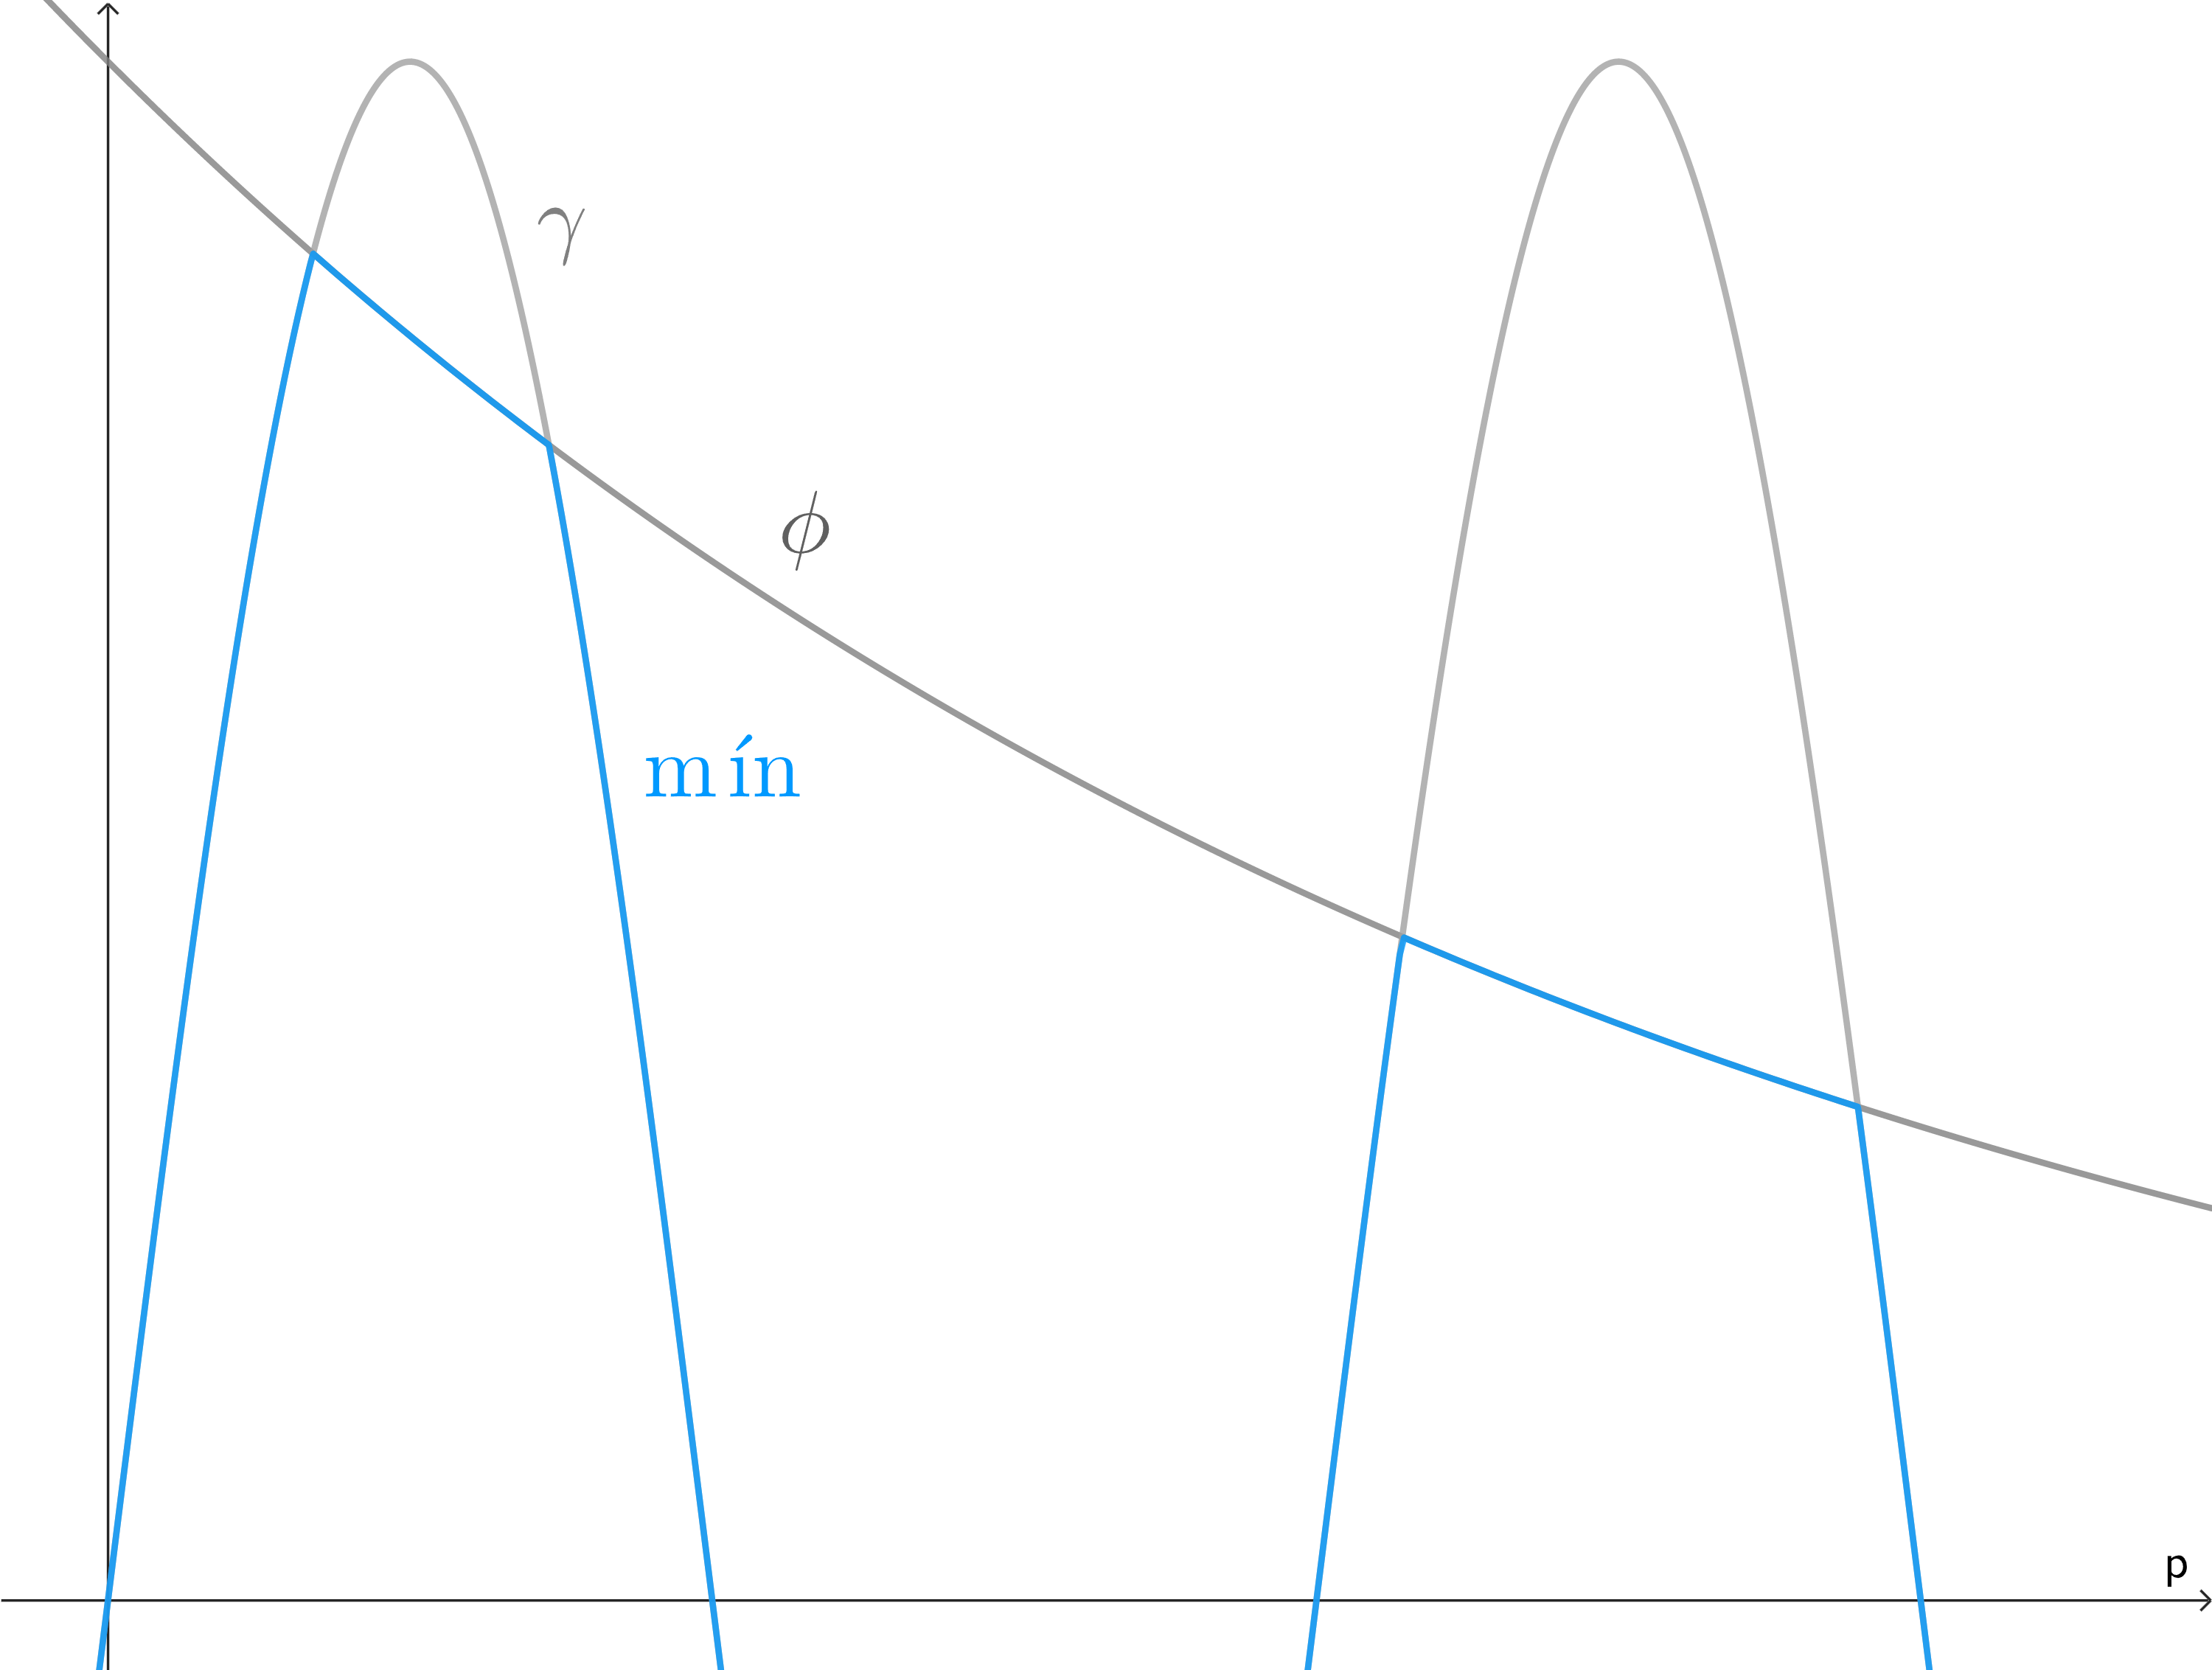
\includegraphics[width=0.75\textwidth]{Plantilla-TFG-master/img/smooth_real.png}
    \caption{Gráfica de $\Min\colon \R\to\R$}
    \label{fig:min_real}
\end{figure}

Para asegurar que $\smin$ sea continua en la frontera de $B_{k}$, imponemos la condición 

\begin{equation*}
    \omega(p) = 0,\ \forall p \in \delta B_{k}.
\end{equation*}

Por otro lado, es lógico que $\omega$ tenga su mayor influencia justo en las intersecciones, luego imponemos también 
\begin{equation*}
    \omega(c) = s, \text{ donde } c \in I \equiv \{p\in\R^3 : \phi(p) = \gamma(p)\},\ s\in \R.
\end{equation*}

El valor $s$ es el que deberemos ajustar para que $\smin$ cumpla nuestros requisitos. Fijado un $p\in B_{k}$, ya tenemos una primera aproximación para $\omega$ :
\begin{equation*}
    \omega(p,k) = s\left( 1-\frac{|\phi(p)-\gamma(p)|}{k} \right)^n = \begin{cases}
        s\left( 1-\frac{\phi(p)-\gamma(p)}{k}\right)^n,\ \phi(p)>\gamma(p), \\[10pt]
        s\left( 1+\frac{\phi(p)-\gamma(p)}{k}\right)^n,\ \phi(p)\le \gamma(p)\\[10pt]
    \end{cases}  ,\ s\in\R,\ n\in\N,
\end{equation*}
donde hemos añadido el parámetro $n$ para añadir más control sobre el resultado final.\newline 
\begin{figure}[!h]
     \begin{minipage}[c]{0.49\linewidth}
        \centering
        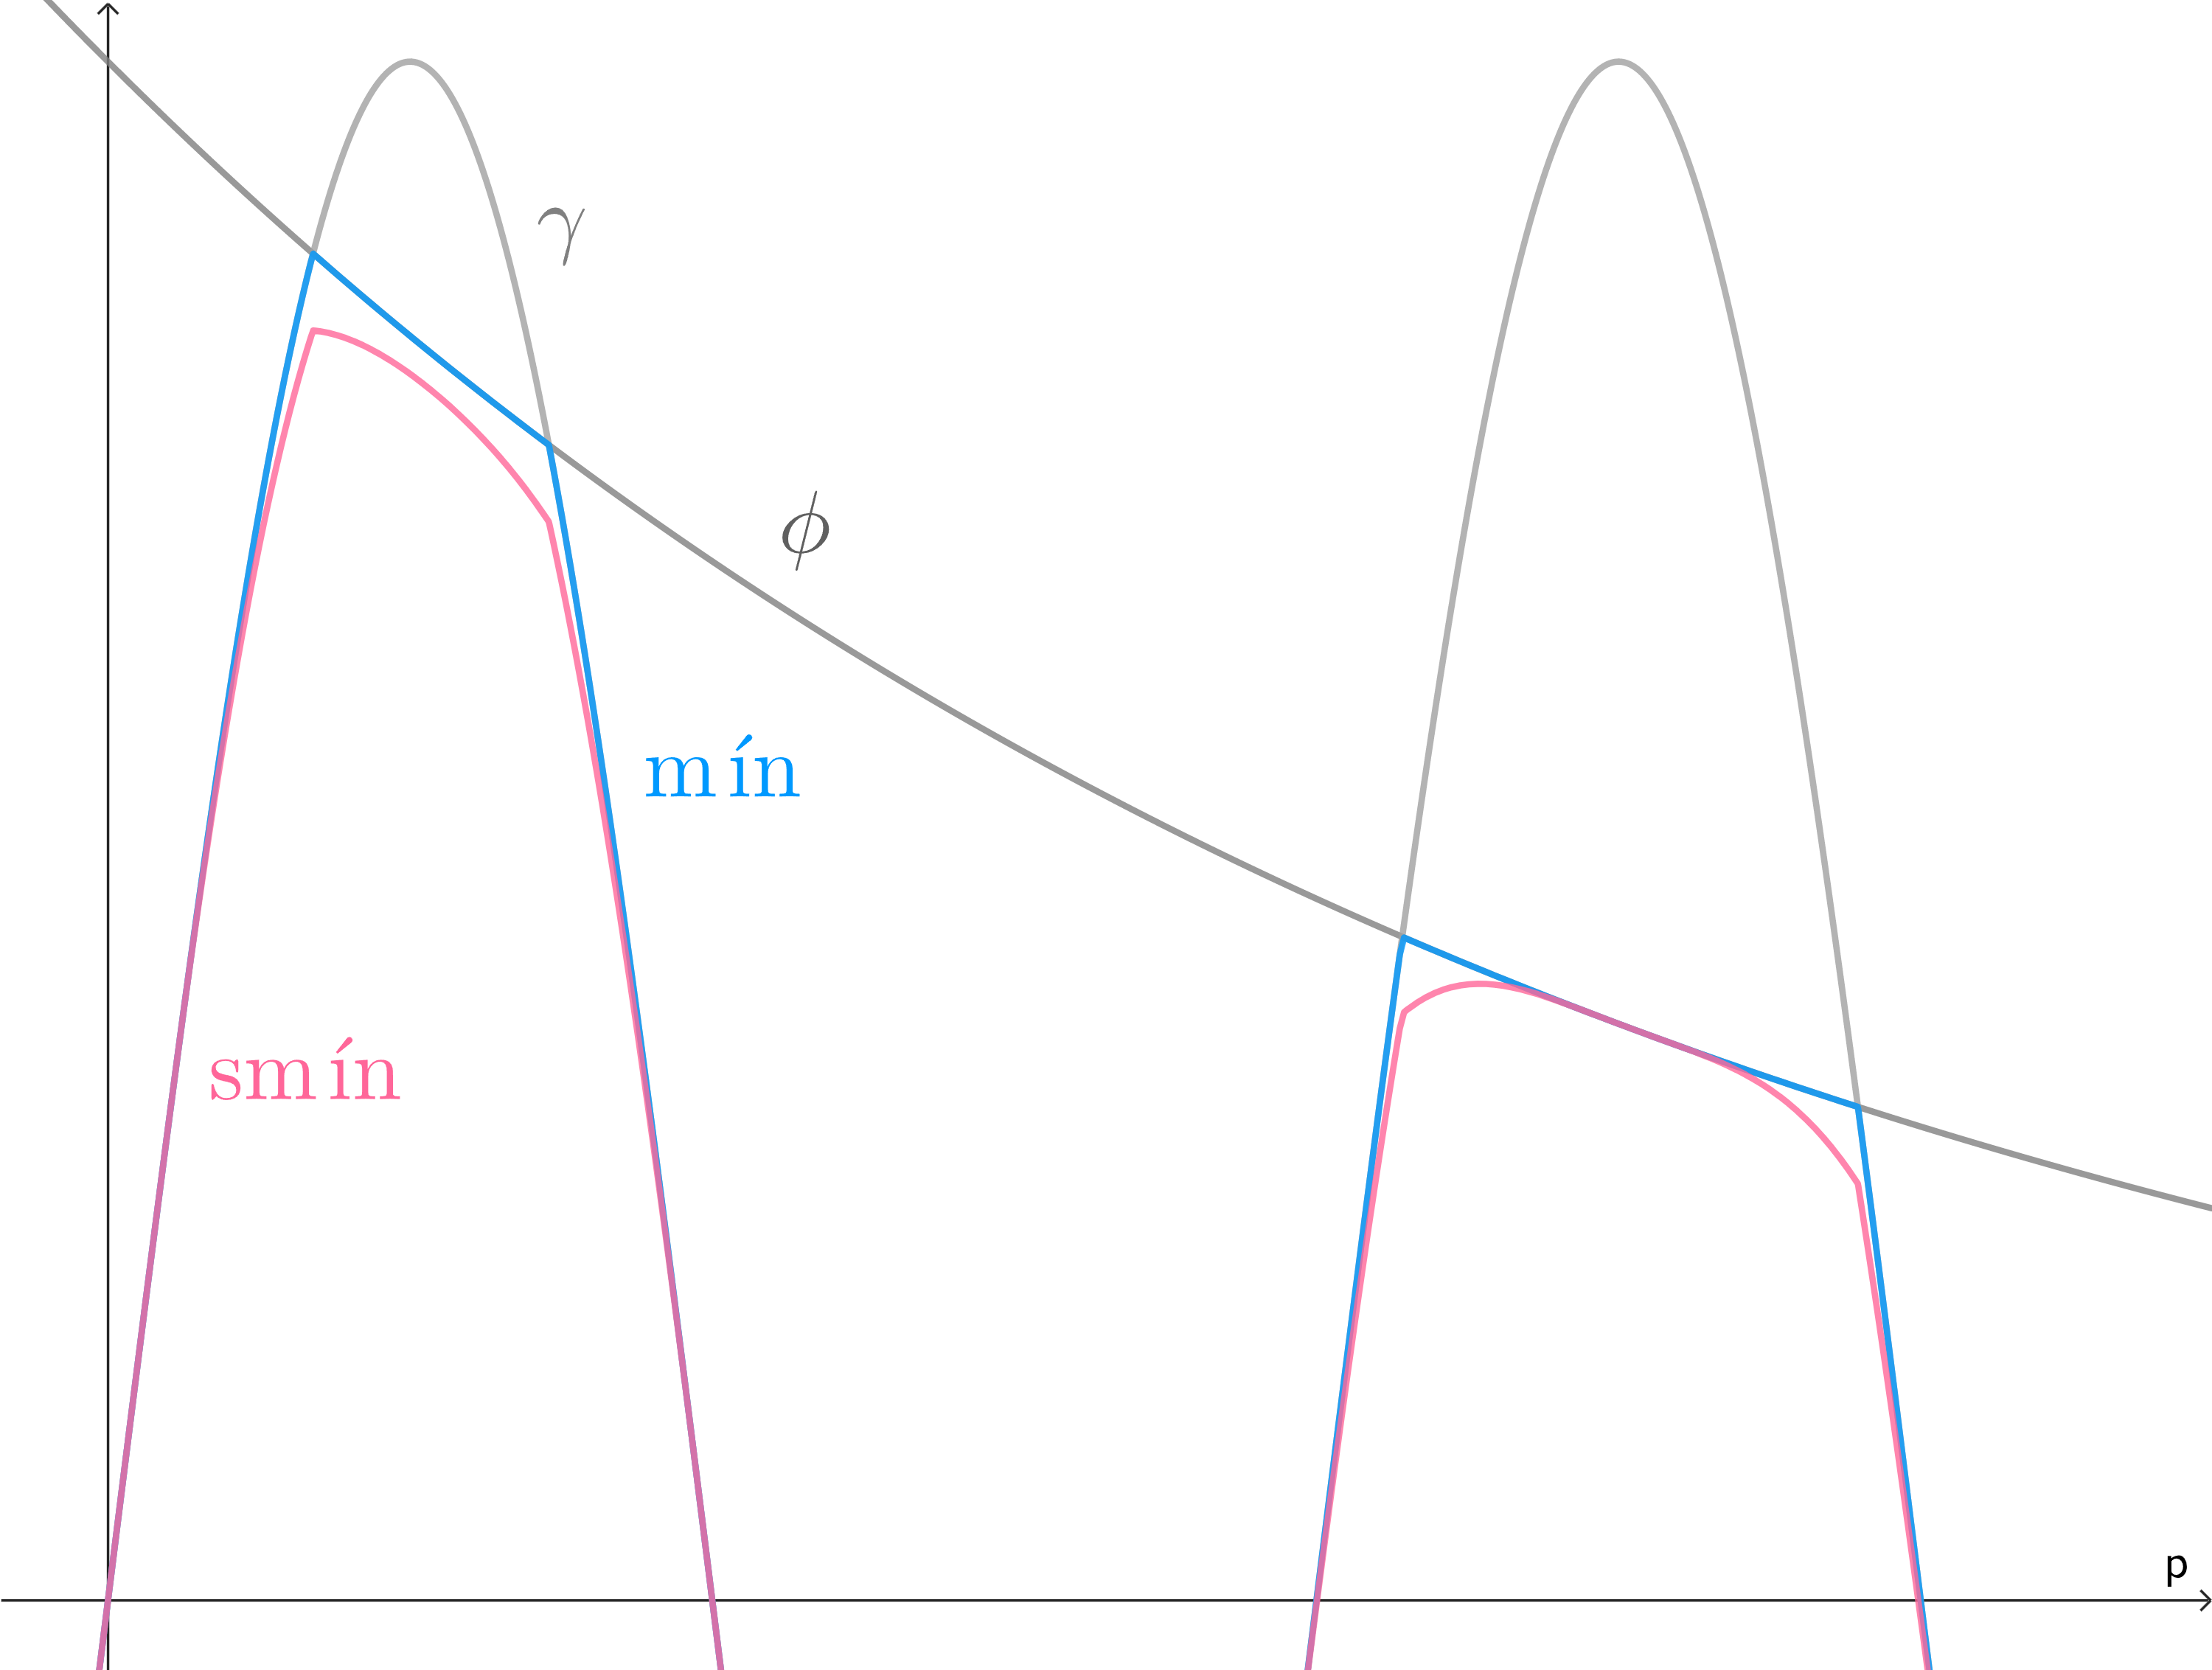
\includegraphics[width=0.95\textwidth]{Plantilla-TFG-master/img/smin_1.png}
        \caption{$k=0.6$}
     \end{minipage}
     \begin{minipage}[c]{0.49\linewidth}
        \centering
        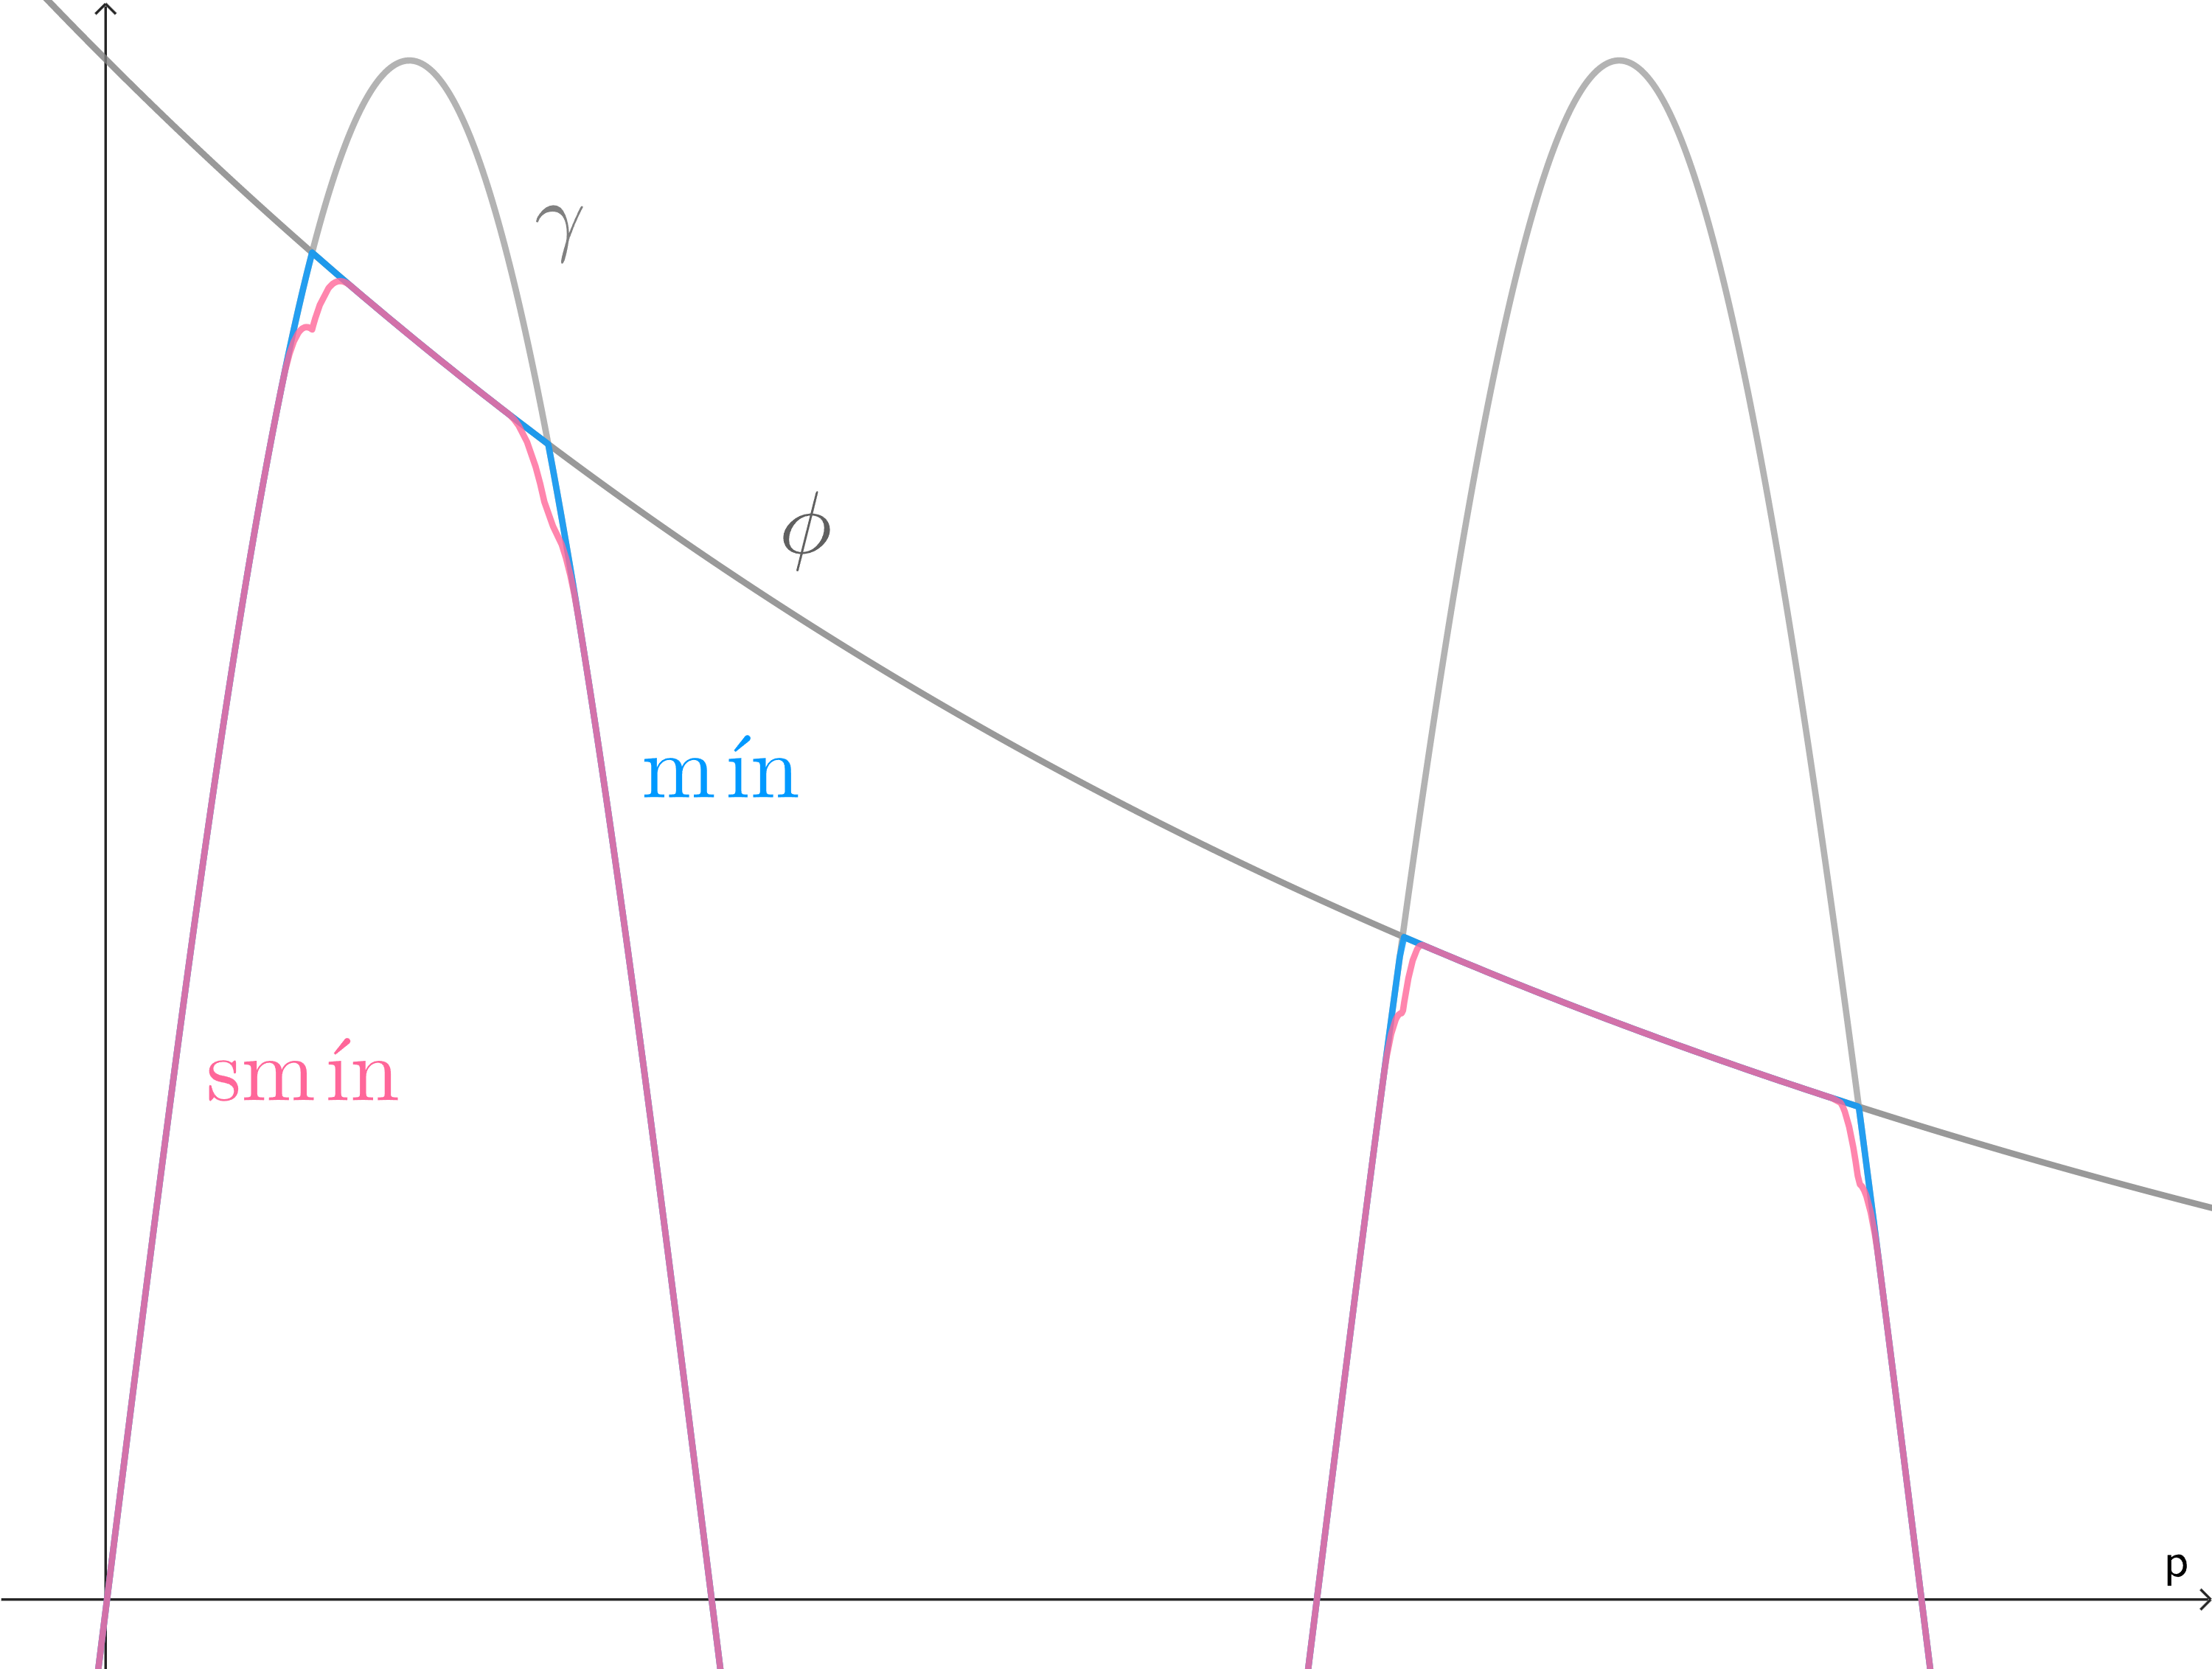
\includegraphics[width=0.95\textwidth]{Plantilla-TFG-master/img/smin_2.png}
        \caption{$k=0.1$}
     \end{minipage}
     \caption{Primera aproximación de $smin(p,k)$ con $s=0.05$ y $n=2$}
     \label{fig:smooth1}
\end{figure}

Es evidente que $\omega$ está bien definida, pues:
\begin{equation*}
    \phi(p)=\gamma(p) \implies \frac{\phi(p)-\gamma(p)}{k} = 0\implies \omega(p) = s
\end{equation*}

Ya podemos pasar a solucionar el problema de continuidad de la derivada. Esta tiene la forma:
\begin{align*}
    \smin'(p,k) &=  \left(\Min(\phi(p),\gamma(p))\right)' - \omega(p,k)'\\[10pt] &= \begin{cases}
        \gamma'(p) + sn\left(1-\frac{\phi(p)-\gamma(p)}{k}\right)^{n-1}\left(\frac{\phi'(p)-\gamma'(p)}{k}\right),\ \phi(p)>\gamma(p), \\[10pt] 
        \phi'(p) - sn\left(1+\frac{\phi(p)-\gamma(p)}{k}\right)^{n-1}\left(\frac{\phi'(p)-\gamma'(p)}{k}\right),\ \phi(p)\le \gamma(p).
    \end{cases}
\end{align*}

Veamos cuándo está bien definida:
\begin{align*}
    \phi' - sn\left(1+\frac{\phi-\gamma}{k}\right)^{n-1}\left(\frac{\phi'-\gamma'}{k}\right) &= \gamma' + sn\left(1-\frac{\phi-\gamma}{k}\right)^{n-1}\left(\frac{\phi'-\gamma'}{k}\right)
\end{align*}

Evaluando en $c\in I$:
\begin{align*}
    \cancel{\phi'(c) -  \gamma'(c)} &= 2sn\left(1+\frac{\phi(c)-\gamma(c)}{k}\right)^{n-1}\left(\frac{\cancel{\phi'(c)-\gamma'(c)}}{k}\right);\\
    s &= \frac{k}{2n}\left(1-\frac{\cancelto{0}{\phi(c)-\gamma(c)}}{k}\right);\\
    s &= \frac{k}{2n}.
\end{align*}
    
Hemos llegado a la expresión final
\begin{align*}
    \omega(p,k) &= \begin{cases}
        \frac{k}{2n}\left( 1-\frac{|\phi(p)-\gamma(p)|}{k} \right)^n,\ &|\phi(p)-\gamma(p)|\le k,\\[10pt]
        0,\ &\text{ otro caso }.
    \end{cases}\\[10pt] &= \frac{\Max\left( k - |\phi(p) - \gamma(p)|, 0\right)^n}{2n\cdot k^{n-1}}  ,\ s\in\R,\ n\in\N.
\end{align*}

Podemos observar los resultados en la \autoref{fig:smooth2}.
\begin{figure}[!h]
     \begin{minipage}[c]{0.49\linewidth}
        \centering
        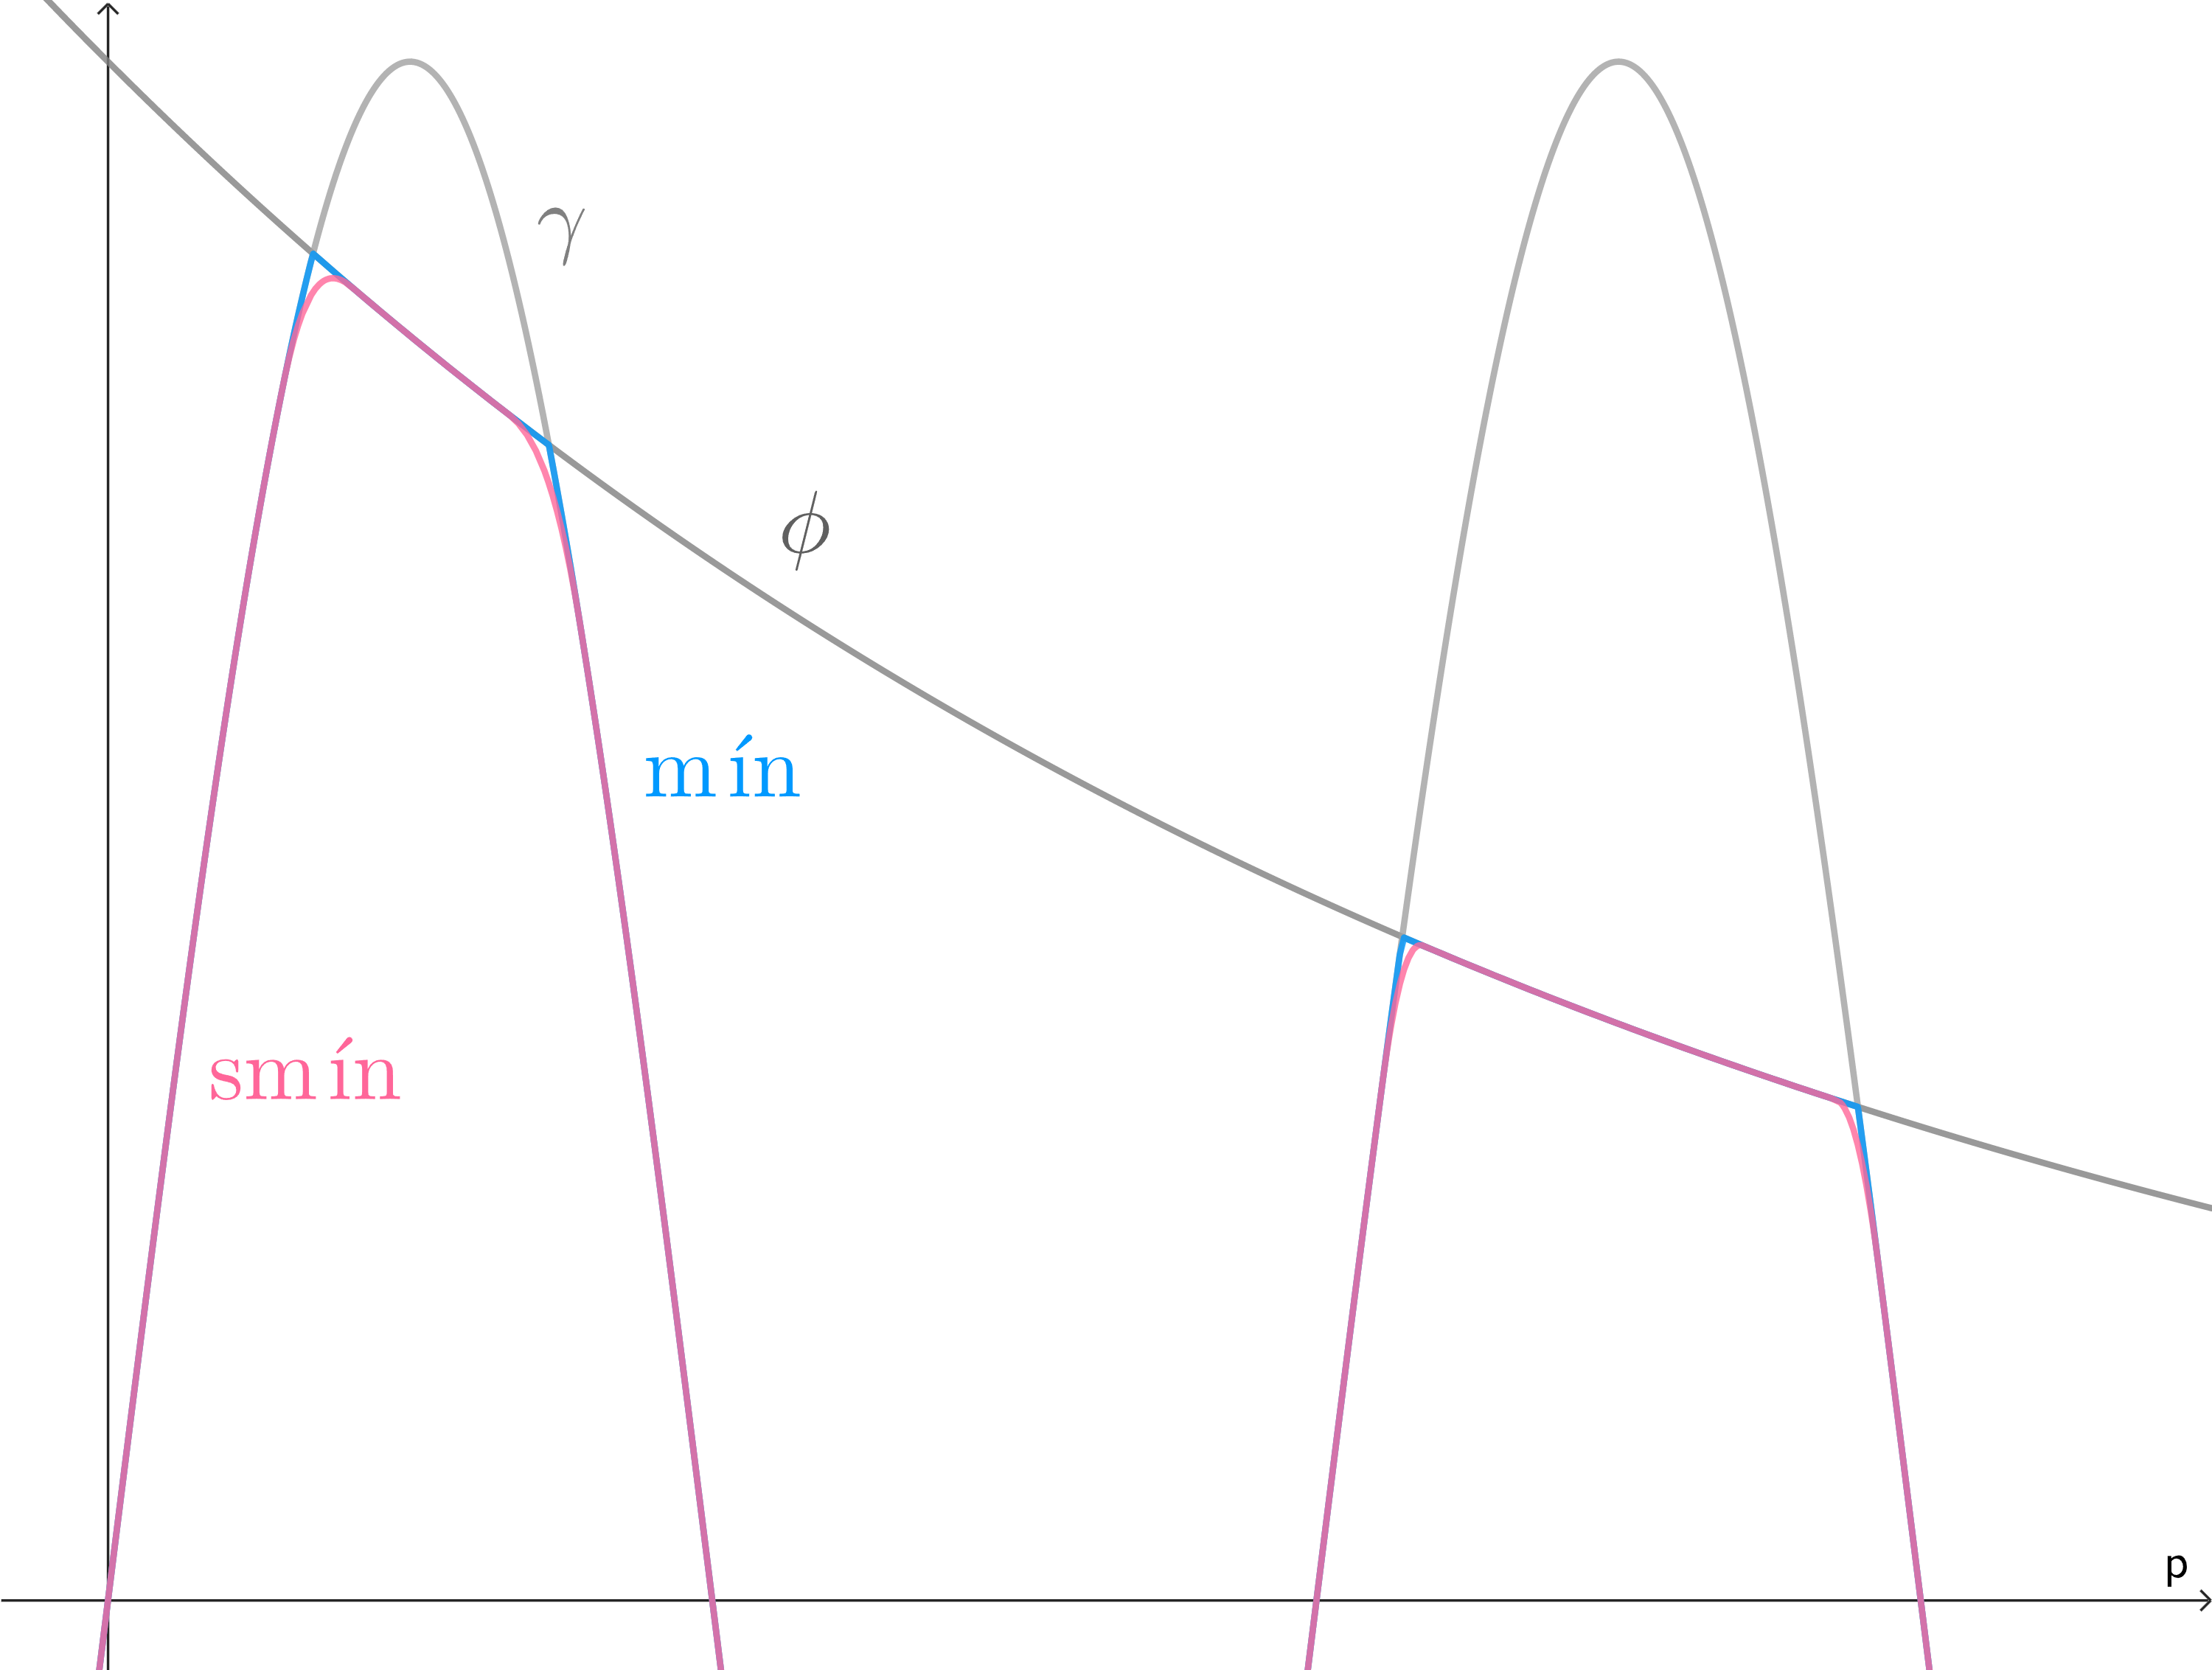
\includegraphics[width=0.95\textwidth]{Plantilla-TFG-master/img/smin_3.png}
        \caption{$k=0.1,\ n=2$}
     \end{minipage}
     \begin{minipage}[c]{0.49\linewidth}
        \centering
        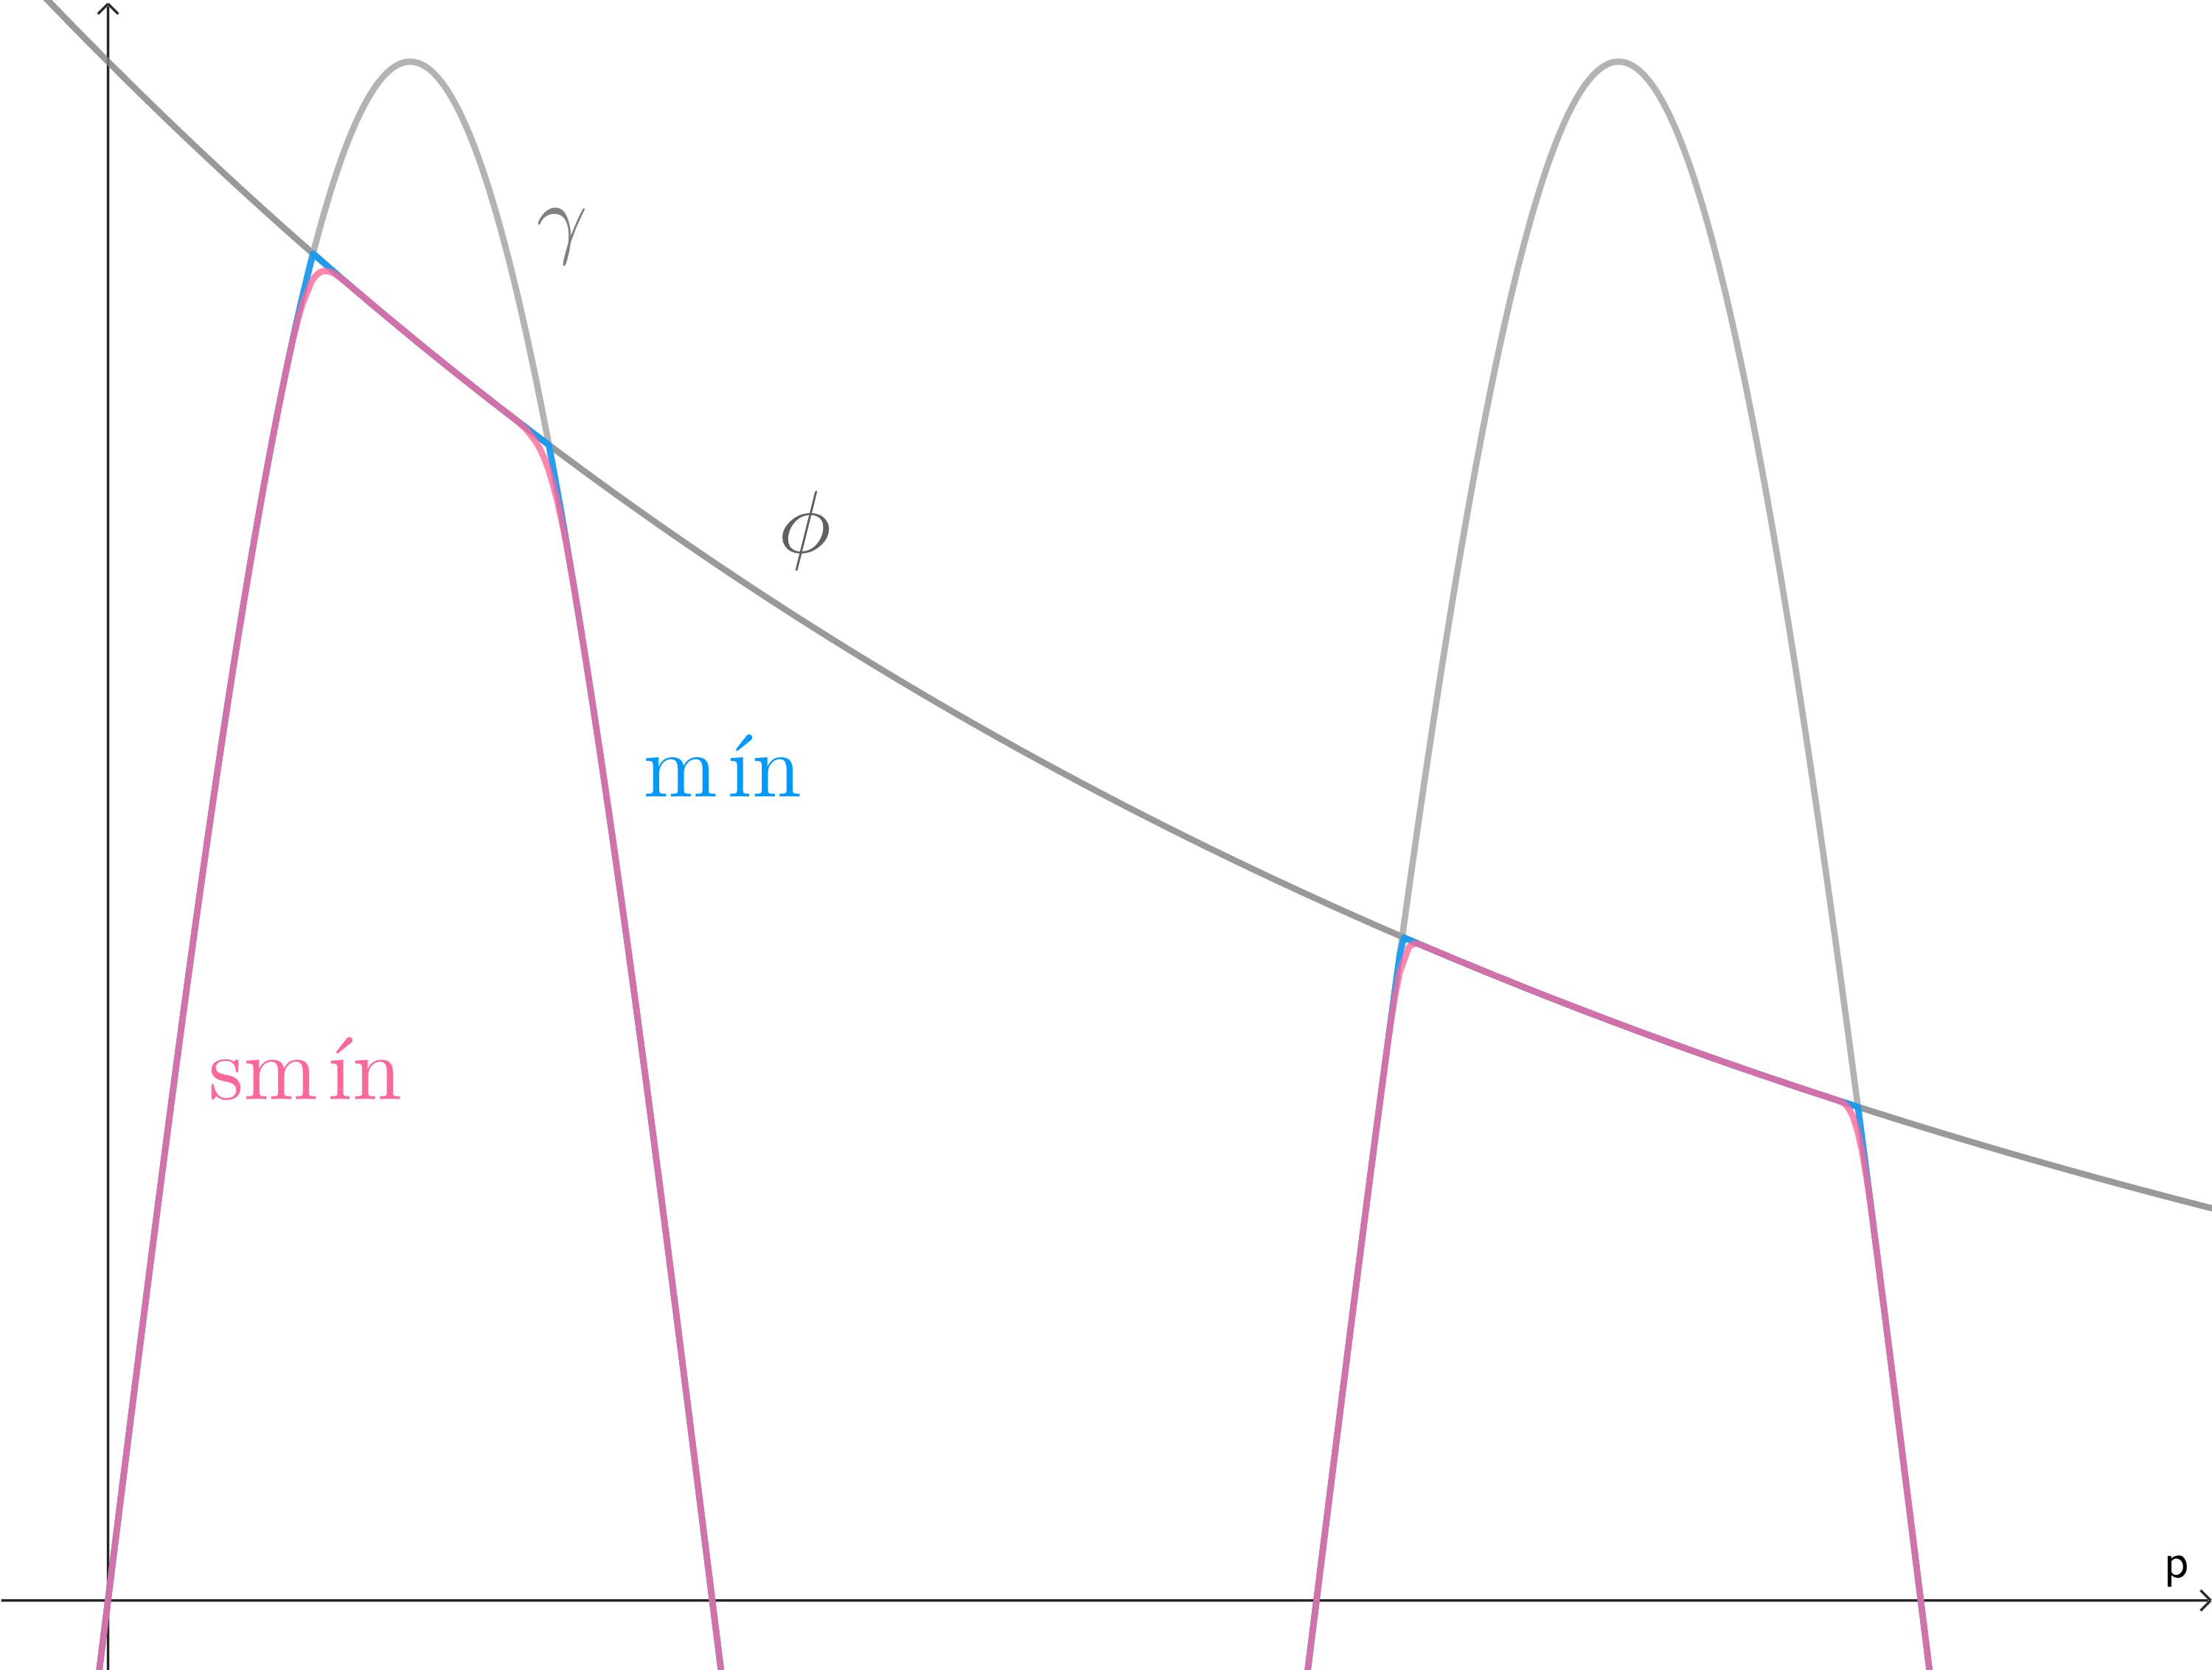
\includegraphics[width=0.95\textwidth]{Plantilla-TFG-master/img/smin_4.png}
        \caption{$k=0.1,\ n=3$}
     \end{minipage}
     \caption{Resultado final de $smin(p,k)$ }
     \label{fig:smooth2}
\end{figure}

Finalmente, para obtener una versión suavizada del máximo, es fácil comprobar que 
\begin{align*}
      \smax_{\phi,\gamma}\colon \R^3\times \R^+_0 &\to \R,\\
      (p,k) &\mapsto -\smin_{-\phi,-\gamma}(p,k).
\end{align*}

Recogemos los resultados obtenidos a continuación.



% Por tanto, dadas $\phi$ y $\gamma$, queremos obtener una versión suavizada de $\Min(\phi,\gamma)$ usando interpolación lineal, que llamaremos $\smin$ y tendrá la forma
% \begin{align*}
%           \smin\colon \R^3 &\to \R^3.\\
%           p &\mapsto h(p)\cdot \phi(p) + (1-h(p))\gamma(p) \text{, donde } h \colon \R^3 \to [0,1].
%     \end{align*}


% Pasamos a buscar $h$. Solo queremos modificar la función en los entornos de los puntos en los que intersecan $\phi$ y $\gamma$, de forma que para el resto de puntos debería ser $h=\{0,1\}$. Los puntos de intersección vienen dados como las soluciones de $m(p)=\gamma(p) - \phi(p)$. Podemos además acotar $m(p)$ en el intervalo $[0,1]$ usando $\Min$ y $\Max$, obteniendo un candidato a valor de $h(p)$:
% \begin{equation}
%     \Min\left(\Max\left(\phi(p)-\gamma(p),0\right),1\right) = \Min\left(\Max\left(m(p),0\right),1\right) \in [0,1]
% \end{equation}

% Sin embargo, podemos ver que la interpolación comienza justo en la intersección, mientras que nos gustaría que esto ocurriese antes. Modificamos la expresión anterior para hacer que la intersección sea el punto medio de la interpolación ($h=0.5$):
% \begin{equation}
%    \Min\left(\Max\left(m(p) + \frac{1}{2},0\right),1\right)
% \end{equation}

% Podemos ver los resultados de esta primera aproximación en la \autoref{fig:smooth1}.

% \begin{figure}[!h]
%      \begin{minipage}[c]{0.49\linewidth}
%         \centering
%         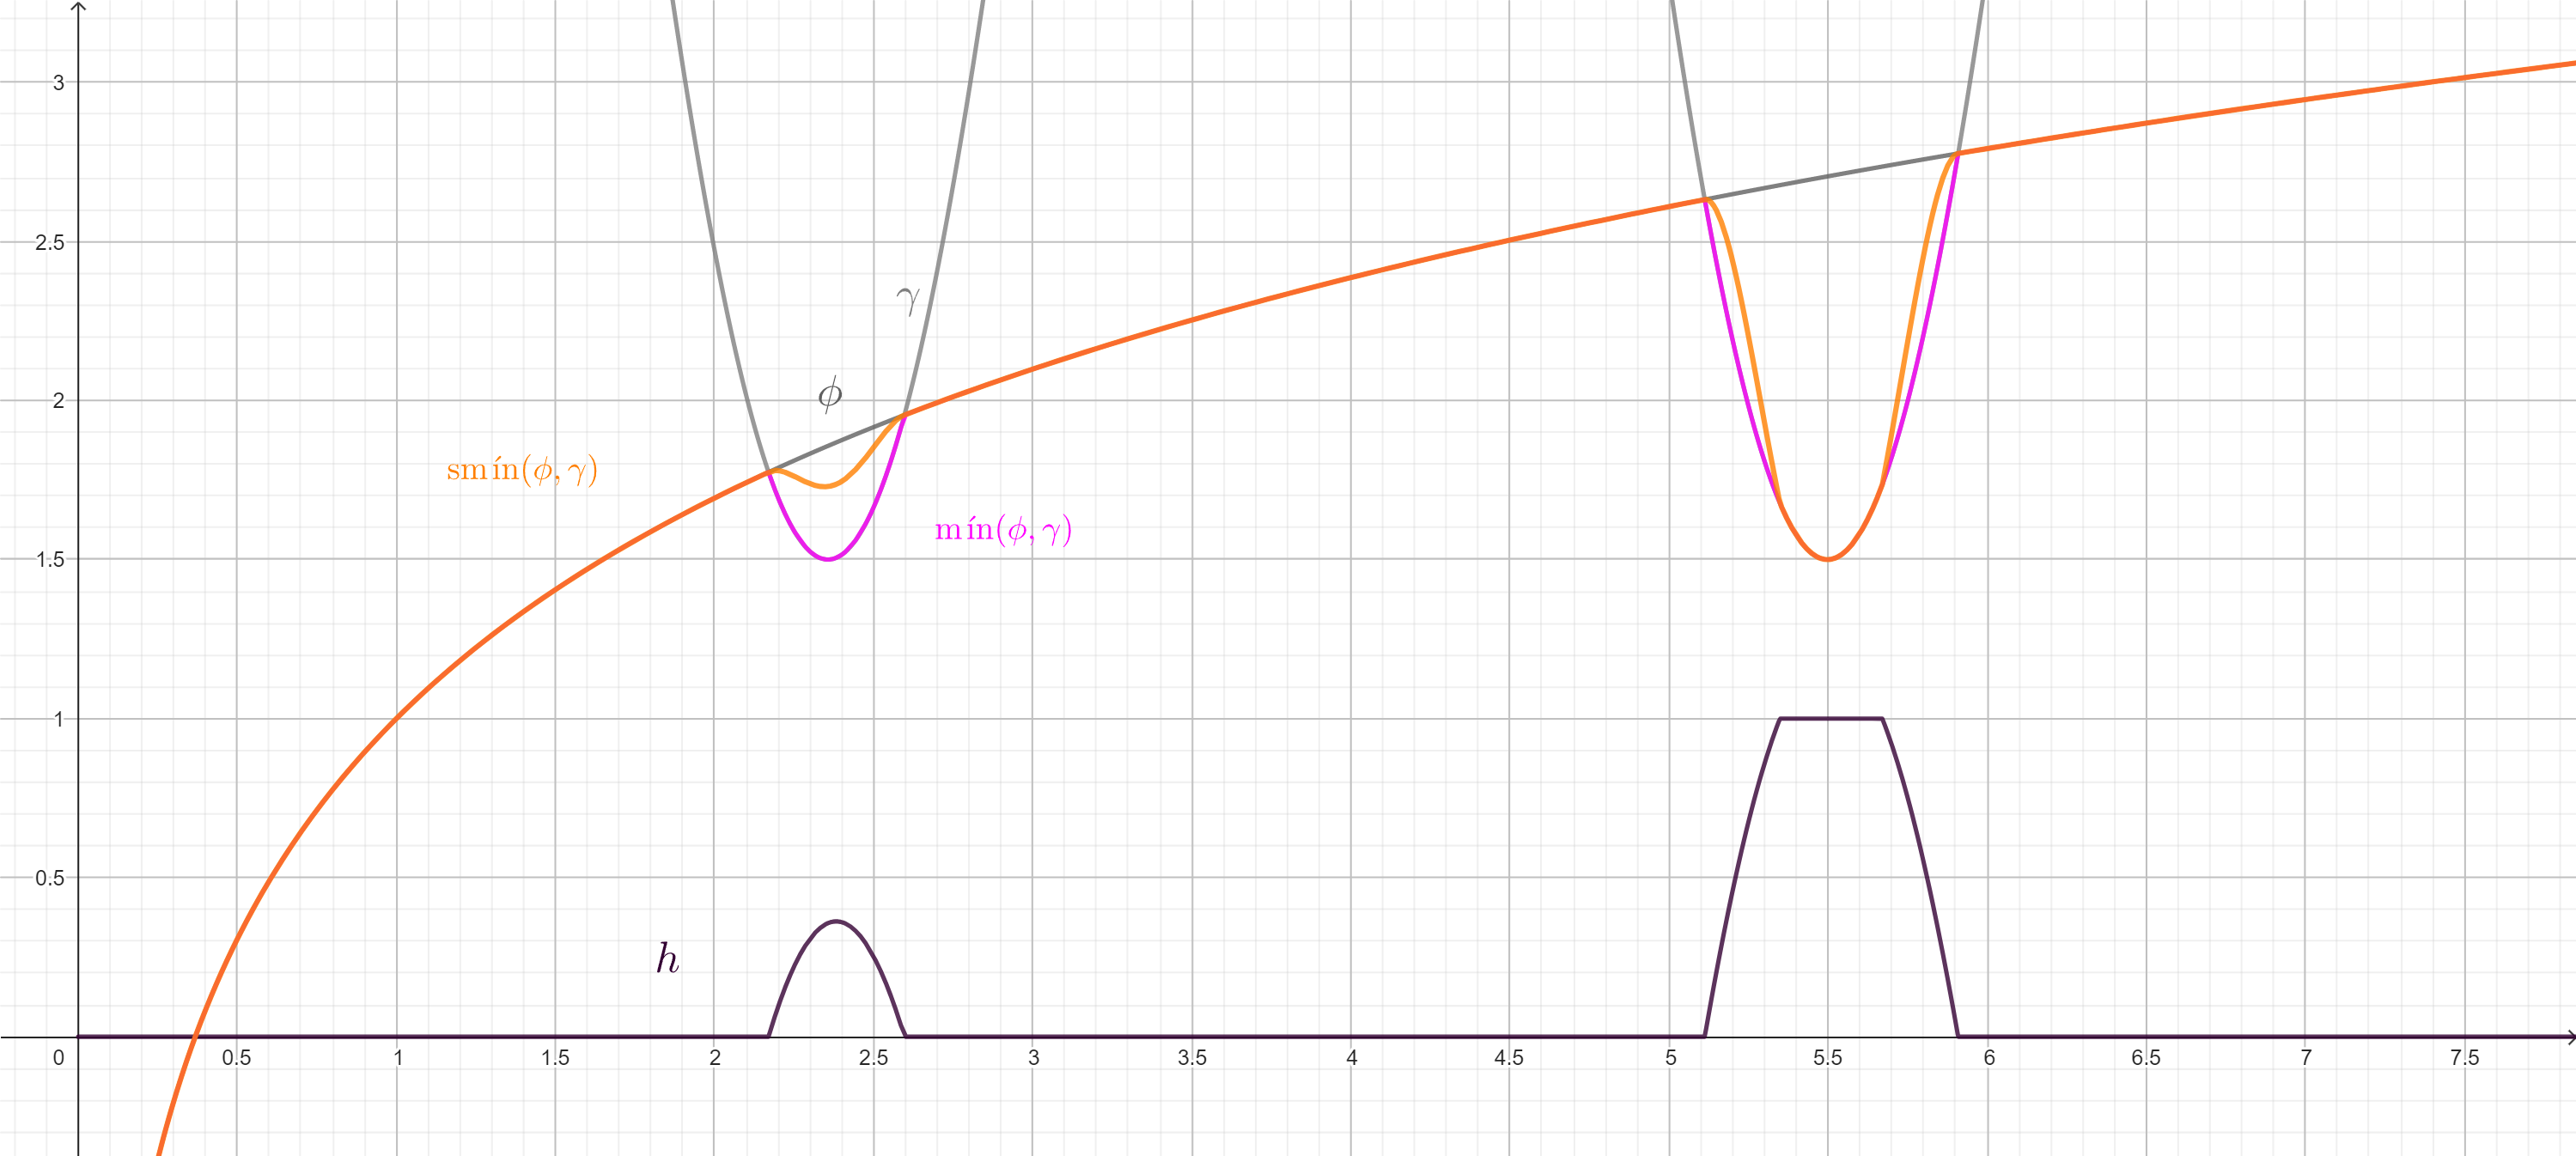
\includegraphics[width=0.95\textwidth]{Plantilla-TFG-master/img/smoothV1_a.png}
%         \caption{$h(p)=0$ en la intersección}
%      \end{minipage}
%      \begin{minipage}[c]{0.49\linewidth}
%         \centering
%         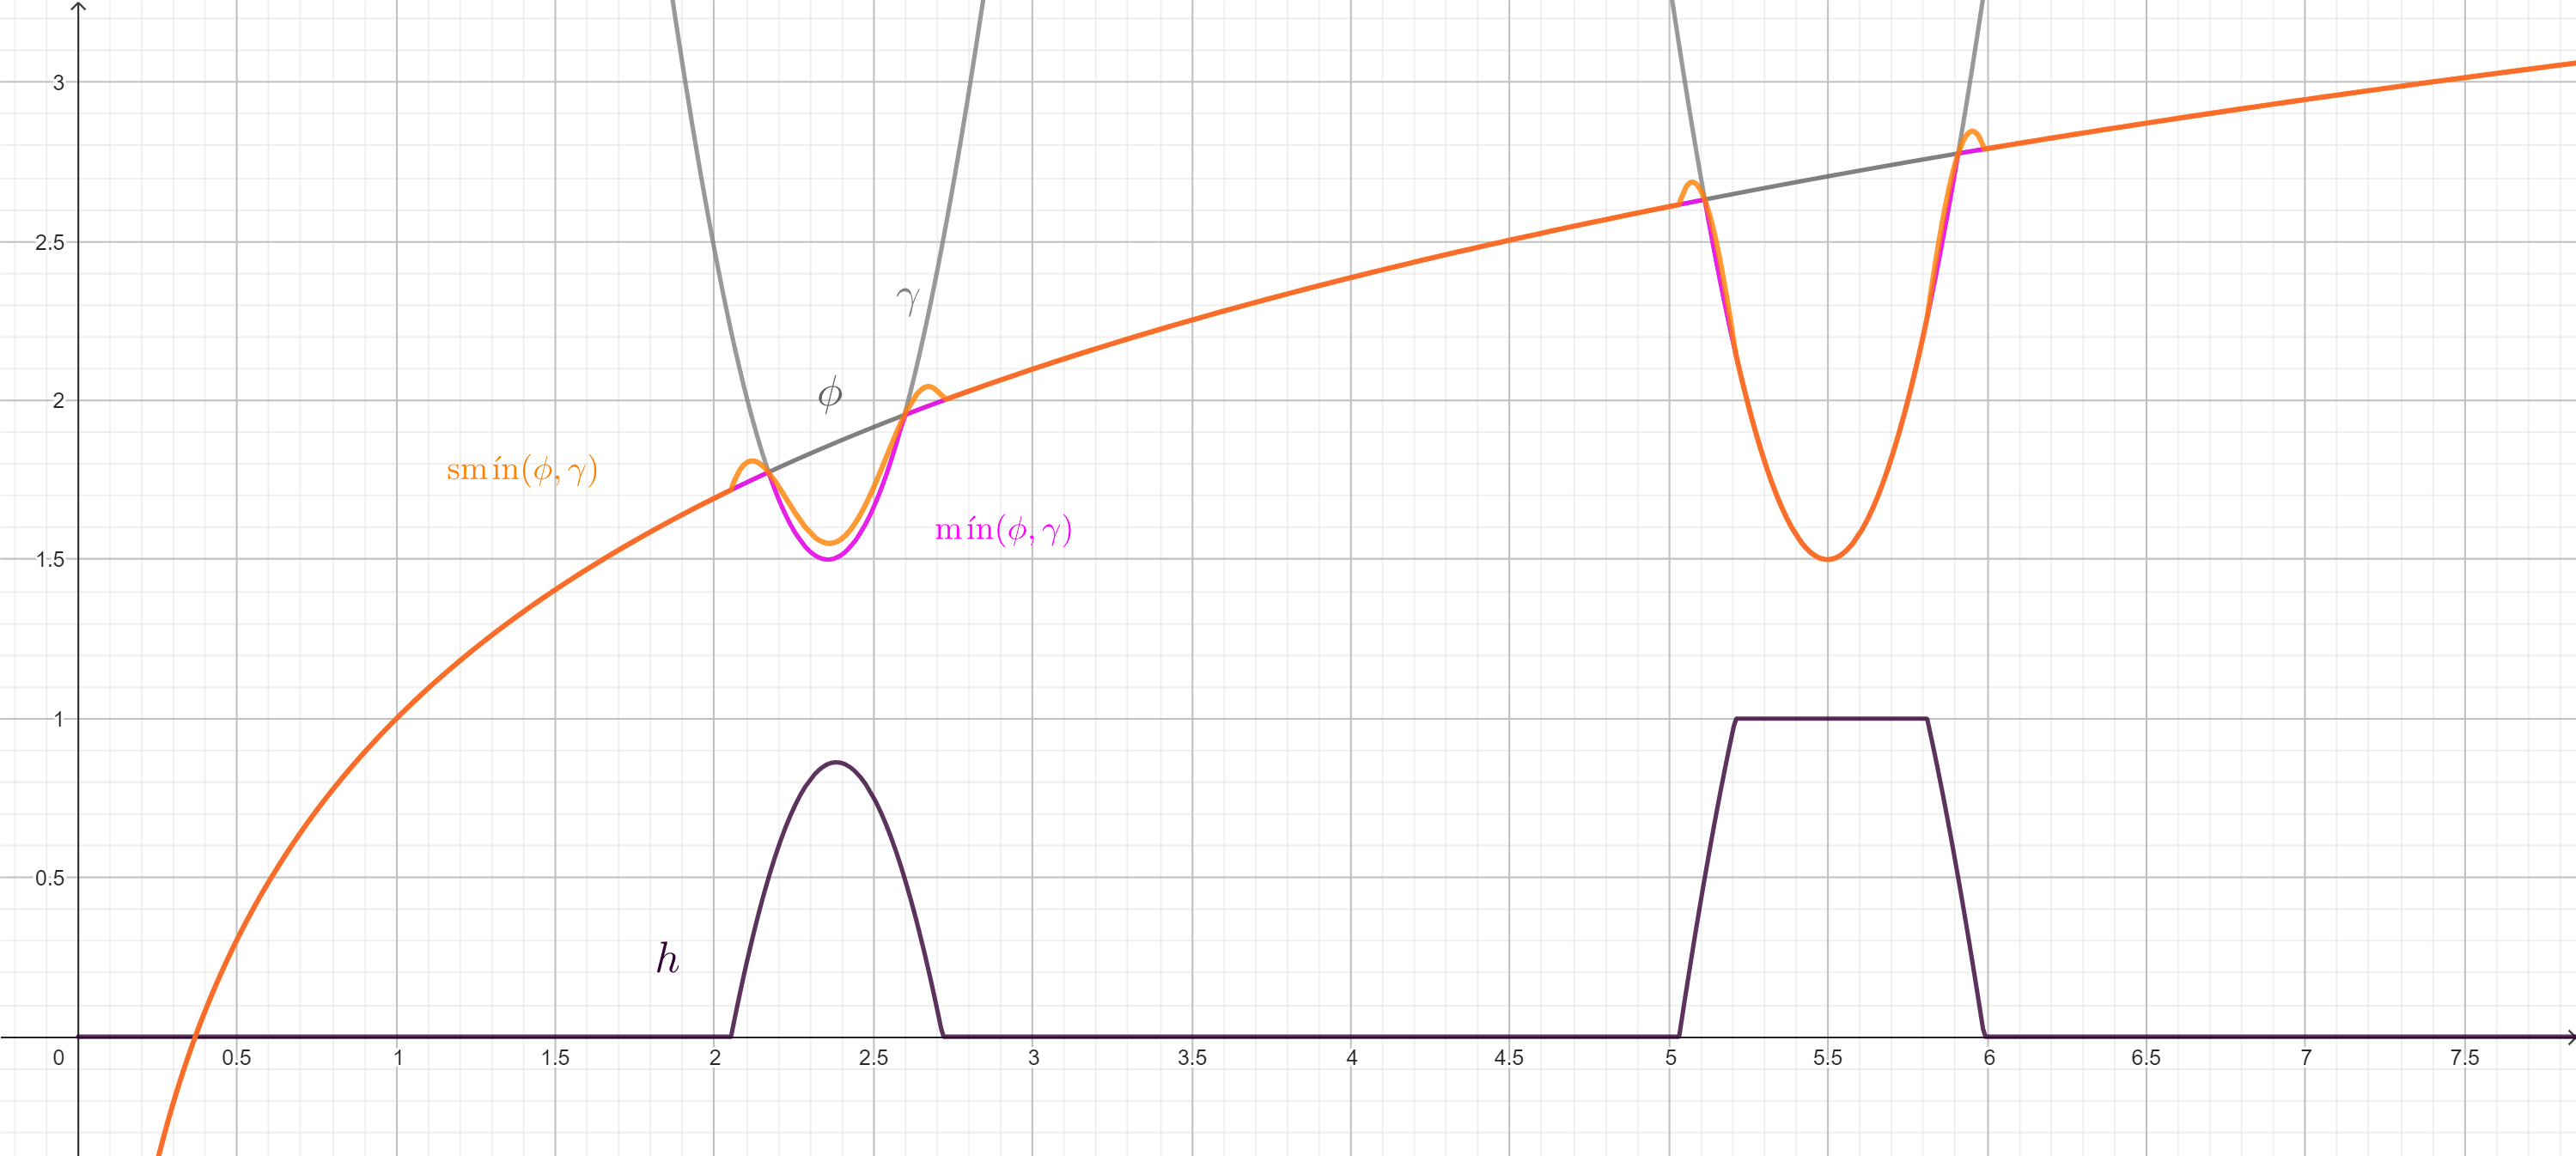
\includegraphics[width=0.95\textwidth]{Plantilla-TFG-master/img/smoothV1_b.png}
%         \caption{$h(p)=0.5$ en la intersección}
%      \end{minipage}
%      \caption{Primera aproximación de la obtención de $h(p)$}
%      \label{fig:smooth1}
% \end{figure}

% Observamos que ahora tenemos un nuevo problema

\begin{definicion}[Operaciones Booleanas Suavizadas]
    Sean $A$ y $B$ isosuperficies generadas por $\phi$ y $\gamma$ respectivamente. Definimos los SDF para las operaciones booleanas suavizadas como sigue.
    \begin{itemize}
        \item \textbf{Unión suavizada: } $\sdf_{unionS}(p) = \Min(\phi(p),\gamma(p)) - \frac{\Max\left( k - |\phi(p) - \gamma(p)|, 0\right)^n}{2n\cdot k^{n-1}}$,
        \item \textbf{Intersección suavizada: } $\sdf_{interS}(p) = -\Min(-\phi(p),-\gamma(p)) + \frac{\Max\left( k - |\phi(p) - \gamma(p)|, 0\right)^n}{2n\cdot k^{n-1}}$,
        \item \textbf{Diferencia suavizada: } $\sdf_{difS}(p) = -\Min(-\phi(p),\gamma(p)) + \frac{\Max\left( k - |\phi(p) + \gamma(p)|, 0\right)^n}{2n\cdot k^{n-1}}$,
    \end{itemize}

    donde $k\in \R^+_0$ controla la influencia del suavizado.        
\end{definicion}

Observamos que los operadores definidos en la \autoref{p:boolean} no son más que un caso particular de estos últimos cuando $k\to 0$.\newline

% \begin{equation*}
%     \lim_{k\to 0} \frac{\Max\left( k - |\phi(p) - \gamma(p)|, 0\right)^n}{2n\cdot k^{n-1}} = \begin{cases}
%         \lim_{k\to 0 } \frac{0}{2n\cdot k^{n-1}} = 0,\ p\notin B_{p,k}\\[10pt]
%          \lim_{k\to 0 } \frac{\left( k - |\phi(p) - \gamma(p)|\right)^n}{2n\cdot k^{n-1}}
%     \end{cases} 
% \end{equation*}


Pasamos ahora a estudiar otro tipo de operaciones, que nos resultarán útiles para generar nuevas formas a partir de un único SDF. Todas ellas se basarán en, dada $\phi$, aplicar una transformación $t:\R^3\to \R^3$ a cada punto de la isosuperficie $S_{\phi}$ para obtener una nueva $S_{\gamma}$. Si queremos saber si un punto $q\in\R^3$ está en $S_{\gamma}$, tenemos que comprobar si su preimagen por la transformación pertenece a $S_{\phi}$. Por tanto, bastará evaluar el SDF original en $t^{-1}(p)$:
\begin{equation*}
    \gamma(p) = \phi(t^{-1}(p)).
\end{equation*}

Esto funciona bien para transformaciones como las traslaciones o rotaciones, ya que mantienen las distancias. Sin embargo, este no es el caso del escalado, ya que si tomamos $l(p) = sp$ con $s\in \R^+_0$:
\begin{equation*}
    \Vert p-p'\Vert = d \implies  \Vert l(p)-l(p')\Vert = \Vert sp-sp'\Vert = s\Vert p-p'\Vert = s\cdot d,\  \text{ donde } p,p' \in S_{\phi}.
\end{equation*}

Como las distancias se escalan, deberemos hacer lo propio con el nuevo SDF, aplicándole el mismo factor de escalado $s$ como muestra la \autoref{d:afines}.

\begin{definicion}[Operaciones afines]\label{d:afines}
    Sea $A$ una isosuperficie. Definimos los SDF para las siguientes operaciones.
    \begin{itemize}
        \item \textbf{Traslación de vector $\boldsymbol{v}$: } $\sdf_{traslacion}(p) = \sdf_{A}(p - v)$,
        \item \textbf{Escalado uniforme de dimensiones $\boldsymbol{s}$: } $\sdf_{escalado}(p) = \sdf_{A}(p/s)\cdot s$,
        \item \textbf{Rotaciones de ángulo $\boldsymbol{\alpha}$ sobre los ejes $\boldsymbol{x,y,z}$: }
        \begin{align*}
            \sdf_{rotX}(p) &= \sdf_{A}(R_x^{-1}(\alpha)\cdot p^t),\ R_x(\alpha) = 
            \begin{pmatrix}
                1&0&0\\
                0&\cos(\alpha) & -\sin(\alpha) \\
                0&\sin(\alpha) & \cos(\alpha) 
                \end{pmatrix},\\[10pt] 
            \sdf_{rotY}(p) &= \sdf_{A}(R_y^{-1}(\alpha)\cdot p^t),\ R_y(\alpha) = \begin{pmatrix}
            \cos(\alpha) &0& \sin(\alpha)\\
            0&1&0\\
            -\sin(\alpha) &0& \cos(\alpha) 
            \end{pmatrix},\\[10pt]
            \sdf_{rotZ}(p) &= \sdf_{A}(R_z^{-1}(\alpha)\cdot p^t),\ R_z(\alpha) = \begin{pmatrix}
            \cos(\alpha) & -\sin(\alpha) & 0\\
            \sin(\alpha) & \cos(\alpha) & 0\\
            0&0&1
            \end{pmatrix}.
        \end{align*}
        
    \end{itemize}
\end{definicion}

Siguiendo el mismo razonamiento, podemos definir operaciones que modifiquen la geometría de la superficie.
\begin{definicion}[Operaciones Deformantes]
    Sea $A$ una isosuperficie. Definimos los SDF para las siguientes operaciones.
    \begin{itemize}
        
        \item \textbf{Torsión: } $\sdf_{torsion}(p) = \sdf_{A}(p')$, con $p' = R_z(ky)\cdot (x,z,y)^t$,
        \item \textbf{Plegado: } $\sdf_{plegado} =\sdf_{A}(p')$, con $p' = R_z(kx)\cdot p^t$,
        \item \textbf{Redondeo: } $\sdf_{redondeo}(p) = \sdf_{A}(p) - k$,
        \item \textbf{Desplazamiento: } $\sdf_{desplazamiento}(p) = \sdf_{A}(\delta(p))$.
    \end{itemize}

    donde
    \begin{itemize}
        \item $k\in \R^+_0$ controla la intensidad de la deformación,
        \item $\delta\colon \R^3\to \R^3$ es un patrón de desplazamiento,
        \item $R_z(\alpha)\in \mathcal{M}_3(\R)$ es la matriz de rotación de ángulo $\alpha$ sobre el eje $z$ dada en la \autoref{d:afines}.
    \end{itemize}
\end{definicion}

Introducimos por último operaciones que permiten generar copias de otras superficies.
\begin{definicion}[Operadores de Posicionamiento]\label{d:posicionamiento}
    Sea $A$ una isosuperficie. Definimos los SDF para las siguientes operaciones.
    \begin{itemize}
        \item \textbf{Simetrías sobre los ejes $\boldsymbol{x,y,z}$:}
        \begin{gather*}
            \sdf_{simX}(p) = \sdf_{A}(\vert x\vert, y, z),\quad \sdf_{simY}(p) = \sdf_{A}(x, \vert y\vert,  z),\\[5pt] \sdf_{simZ}(p) = \sdf_{A}(x,y,\vert z\vert),
        \end{gather*}
        \item \textbf{Simetrías sobre los planos $\boldsymbol{xy,xz,yz}$:}
        \begin{gather*}
            \sdf_{simXY}(p) = \sdf_{A}(\vert x\vert, \vert y\vert, z),\quad \sdf_{simXZ}(p) = \sdf_{A}(\vert x\vert, y,  \vert z\vert),\\[5pt]\sdf_{simYZ}(p) = \sdf_{A}(x,\vert y\vert ,\vert z\vert),
        \end{gather*}
        \item \textbf{Repetición $\boldsymbol{l\in \N^3}$ veces en los ejes $\boldsymbol{x,y,z}$ con separación $\boldsymbol{s\in\R}$:} 
        \begin{equation*}
            \sdf_{rep}(p) = \sdf_{A}(p - s\cdot c\left(r\left(\frac{p}{s}\right), -l, l\right),
        \end{equation*}
        \item \textbf{Repetición infinita:}
        \begin{equation*}
            \sdf_{repInf}(p) = \sdf_{A}\left((p+\frac{l}{2}\mod l )- \frac{l}{2}\right),
        \end{equation*}
    \end{itemize}
    donde
    \begin{itemize}
        \item $c\colon \R\times\R\times\R\to \R,\ c(x,a,b) = \Min(\Max(x, a), b)$ acota $x$ en $[a,b]$,
        \item $r\colon \R^3 \to \R^3$ redondea las componentes de un vector a sus enteros más cercanos.
    \end{itemize}
\end{definicion}

\begin{observacion}
    Hay casos en los que los SDF definidos en la \autoref{d:posicionamiento} podrían no ser exactos, al igual que ocurría con la intersección y la diferencia en la \autoref{p:boolean}:
    \begin{itemize}
        \item Para las simetrías, cuando el objeto interseca el plano de simetría,
        \item Para las repeticiones, cuando las dimensiones del objeto sean mayores o iguales a $l/2$.
    \end{itemize}
\end{observacion}

A la vista de todas esta operaciones a nuestra disposición, es evidente el potencial que tienen los SDF, tanto en la generación y modificación de figuras como en su eficiencia, ya que podemos visualizar miles de objetos al precio de uno utilizando las simetrías o repeticiones.\newline

En el \autoref{ap:operacionesSDF} se muestra el resultado de aplicar las operaciones vistas a diferentes primitivas.

\section{Renderizado}
Una vez definida la escena a partir de un SDF, necesitamos una forma para visualizarla, para lo que utilizaremos la API de OpenGL \cite{opengl} y aplicaremos la técnica de \textit{raymarcing}. 

\subsection{Creación del lienzo}
Si bien se puede hacer \textit{raymarching} directamente sobre una escena 3D, nuestra escena constará únicamente de un plano formado por cuatro vértices y dos triángulos, que usaremos como lienzo  (o \textit{canvas}) para dibujar sobre él. Para ello, necesitaremos trabajar sobre diferentes espacios de coordenadas que nos proporciona OpenGL, los cuales pasamos a enumerar.
\begin{itemize}
    \item \textbf{Coordenadas locales o de objeto:} distancias relativas al origen del objeto,
    \item \textbf{Coordenadas globales o de mundo:} distancias relativas a un origen común para todos los objetos,
    \item \textbf{Coordenadas de cámara:} distancias relativas a un sistema de referencia posicionado y alineado con la cámara,
    \item \textbf{Coordenadas de recortado:} distancias normalizadas en el rango $[-1,1]^2$ relativas a un sistema asociado al rectángulo que forma la imagen en pantalla.
\end{itemize}

Para crear el lienzo, debemos declarar sus vértices y cómo estos se unen formando triángulos. Si hacemos uso de \texttt{GL\_TRIANGLES} bastará con definir los vértices en sentido antihorario, pero hay que tener en cuenta que tendremos que repetir dos vértices, ya que se irán formando los triángulos en grupos de tres vértices. Una alternativa para no repetir vértices sería utilizar tablas de vértices e índices, pero en nuestro caso no merece la pena al tener únicamente seis vértices. Un ejemplo de definición de vértices formando un lienzo rectangular podría ser el que se muestra en la \autoref{fig:canvas}.

\begin{figure}[ht]
    \centering
    \begin{minipage}{0.50\textwidth}
        \begin{lstlisting}
glBegin(GL_TRIANGLES);
    glColor3f(1.0f, 1.0f, 1.0f); 
    
    // Triangulo inferior
    glVertex3f(-2.0f, -1.0f, 0.0f);
    glVertex3f(-2.0f, 1.0f, 0.0f);
    glVertex3f(2.0f, 1.0f, 0.0f);
    
    // Triangulo superior
    glVertex3f(-2.0f, -1.0f, 0.0f);
    glVertex3f(2.0f, 1.0f, 0.0f);
    glVertex3f(2.0f, -1.0f, 0.0f);
glEnd();
\end{lstlisting}
    \end{minipage}%
    \hfill
    \begin{minipage}{0.40\textwidth}
        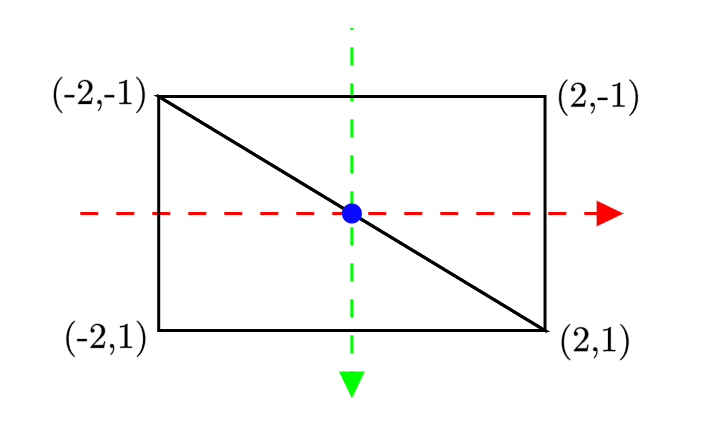
\includegraphics[width=\textwidth]{canvas.png}
    \end{minipage}
    
    
    \caption{Construcción del lienzo}
    \label{fig:canvas}
\end{figure}


Este lienzo, como toda geometría, tendrá asignado dos \textit{shaders} o procesadores, programas escritos en GLSL (lenguaje parecido a C) y que se ejecutan en la GPU. Estos programas son independientes entre sí, y la única forma en la que pueden comunicarse entre ellos es mediante el paso de atributos de entrada y salida con las palabras clave \texttt{in} y \texttt{out} respectivamente. Hay dos tipos de \textit{shaders}: de vértices (\textit{vertex shader}) y de fragmento o píxel (\textit{fragment shader}), cada uno con atributos específicos de entrada y salida.\newline

En el \textit{vertex shader} utlizaremos
\begin{itemize}    
    \item \textbf{\texttt{in vec4 gl\_Vertex}}: contiene las coordenadas locales del vértice actual y es pasado autómaticamente por la aplicación,
    \item \textbf{\texttt{out vec4 gl\_Position}}: posición transformada del vértice actual. La cuarta componente es la componente homogénea, que es necesaria para realizar el cambio a coordenadas recortadas.
\end{itemize}
En el \textit{fragment shader} utilizaremos
\begin{itemize}
    \item \textbf{\texttt{in vec4 gl\_FragCoord}}: coordenadas de dispositivo para el píxel actual en el \textit{fragment shader}. Al ser un atributo de entrada del \textit{fragment shader}, está interpolada en cada vértice. La cuarta componente es la inversa de la componente homogénea de \texttt{gl\_Position}, y se utiliza en el cálculo de la profundidad de los píxeles y en las operaciones de corrección de perspectiva,
    \item \textbf{\texttt{out vec4 gl\_FragColor}}: terna RGBA para asignar el color del píxel actual en el \textit{fragment shader}.
\end{itemize}
Por último, en caso de que queramos pasar nuestros propios atributos desde otro programa, deberemos hacerlo a través de un \texttt{uniform}.\newline

En primer lugar se ejecuta el \textbf{procesador de vértices o \textit{vertex shader}} para cada vértice de la geometría. Su objetivo principal es el de realizar transformaciones de coordenadas, y adicionalmente pasar atributos al \textit{fragment shader}. Dada la posición del vértice actual, que se nos proporciona a través del atributo \texttt{gl\_Vertex}, para cambiar de un sistema de coordenadas a otro se utilizan matrices de transformación \cite{article:matrices} \cite{article:matrices2}. En particular, usaremos las que siguen.
\begin{figure}[h]
    \centering
    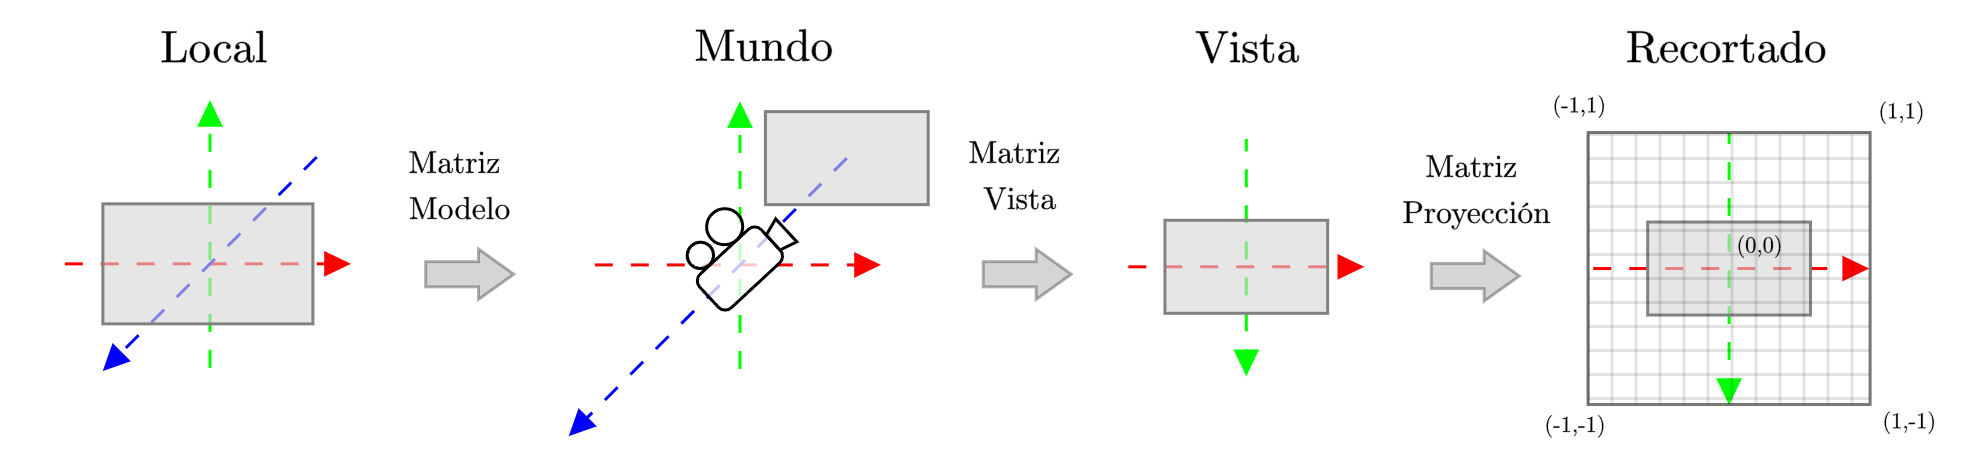
\includegraphics[width=\textwidth]{Plantilla-TFG-master/img/matrices2.png}
    \caption{Coordenadas locales a recortadas}
    \label{fig:matrices}
\end{figure}
\begin{itemize}
    \item \textbf{Matriz de modelo $\boldsymbol{M}$:} define la posición, orientación y escala del objeto en la escena. Se utiliza para pasar del coordenadas locales a coordenadas de mundo. En nuestro caso, si creamos el plano centrado en el origen, podemos simplemente tomar
    \begin{equation*}
        M = Id_{4},
    \end{equation*}
    \item \textbf{Matriz de vista  $\boldsymbol{V}$:} define la posición y orientación de cada punto respecto a la cámara de la escena. Se utiliza para pasar de coordenadas de mundo a coordenadas de vista. Lo que ocurre en realidad es que la cámara está fija en el origen, y es el resto de la escena es la que se mueve respecto a ella. Por tanto, esta matriz contiene la posición y orientación inversa de la cámara. En nuestro caso, si queremos desplazar la cámara una unidad en el eje Z, la matriz de vista tendrá la forma
    \begin{equation*}
        V = \begin{pmatrix}
        1 & 0 & 0 & 0\\
        0 & 1 & 0 & 0\\
        0 & 0 & 1 & -1\\
        0 & 0 & 0 & 1
        \end{pmatrix},
    \end{equation*}
    
    \item \textbf{Matriz de proyección:} define cómo la escena se proyecta en la pantalla, incluyendo el campo de visión, aspecto y planos cercano y lejano. Se utiliza para pasar de coordenadas de vista a coordenadas recortadas. OpenGL nos proporciona una función para calcularla:
    \begin{lstlisting}
    glm::mat4 projectionMatrix = glm::perspective(
        glm::radians(FoV),  // campo vertical de vision
        4.0f / 3.0f,         // aspecto
        0.1f,                // plano de corte cercano
        100.0f               // plano de corte lejano
    );
    \end{lstlisting}
    % \item \textbf{Matriz de ventana o \textit{viewport}:} se transforman las coordenadas de recortado a las coordenadas de dispositivo. Estas coordenadas están centradas en la esquina inferior izquierda de la pantalla y están en el rango $[0,r_x]\times [0,r_y]$, donde $r=(r_x,r_y)$ es la resolución de la pantalla.
\end{itemize}

Con esto, ya podemos escribir nuestro \textit{vertex shader}:
\begin{lstlisting}[title=Procesador de vértices]
#version 330    
uniform mat4 projection;
uniform mat4 view;
uniform mat4 model;

void main()
{
    gl_Position = projection * view * model * gl_Vertex;
}
\end{lstlisting}

Tras realizar estas transformaciones, las coordenadas de recortado se transforman a coordenadas de dispositivo, que están centradas en la esquina inferior izquierda de la pantalla y toman valor en el rango $[0,r_x]\times [0,r_y]$, donde $r=(r_x,r_y)$ es la resolución de la pantalla.\newline

Ahora le toca el turno al \textbf{procesador de fragmentos o \textit{fragment shader}}. Este se ejecuta para cada píxel de la pantalla, y su objetivo es asignar a la variable \texttt{gl\_FragColor} el color que el píxel tendrá como una terna RGBA. Será aquí donde hagamos todos los cálculos necesarios pare renderizar la superficie con \textit{raymarching}. Para ello, necesitaremos un sistema de coordenadas dentro del propio lienzo, que generaremos haciendo uso de \texttt{gl\_FragCoord} y la resolución del lienzo, atributo que pasaremos nosotros al \textit{shader} a través de un \texttt{uniform}, que llamaremos \texttt{u\_resolution}.

Para obtener estas coordenadas, primero desplazamos el origen que nos proporciona \texttt{gl\_FragCoord} al centro de la pantalla, y posteriormente normalizamos respecto a alguno de los ejes. Hacemos esto porque si intentamos normalizar sobre ambos ejes, obtendremos coordenadas en el rango $[-0.5,0.5]^2$, lo que hará que en un lienzo que no sea cuadrado, la imagen se vea estirada en la dirección del eje más largo. Nosotros normalizaremos respecto al eje vertical, ya que en nuestro caso será siempre el menor. Esto nos dará como resultado unas coordenadas con valores en $\left[ -0.5\cdot aspect, 0.5\cdot aspect \right] \times [-0.5, 0.5]$, donde $aspect$ es el ratio de aspecto del lienzo:

\begin{equation*}
    uv = \frac{gl\_FragCoord.xy - 0.5\cdot u\_resolution.xy}{u\_resolution.y} ,
\end{equation*}

Hemos denotado a las coordenadas obtenidas como \texttt{uv}, haciendo referencia a la similitud que tienen con el uso que se le da a las coordenadas de textura habituales. Podemos ver la diferencia entre ambos sistemas de coordenadas si usamos \texttt{uv} como los canales rojo y verde de \texttt{gl\_FragColor}, tal y como se muestra en la \autoref{fig:uv}.\newline

\begin{figure}[htbp]
    \centering
    \begin{minipage}[b]{0.45\textwidth}
        \centering
        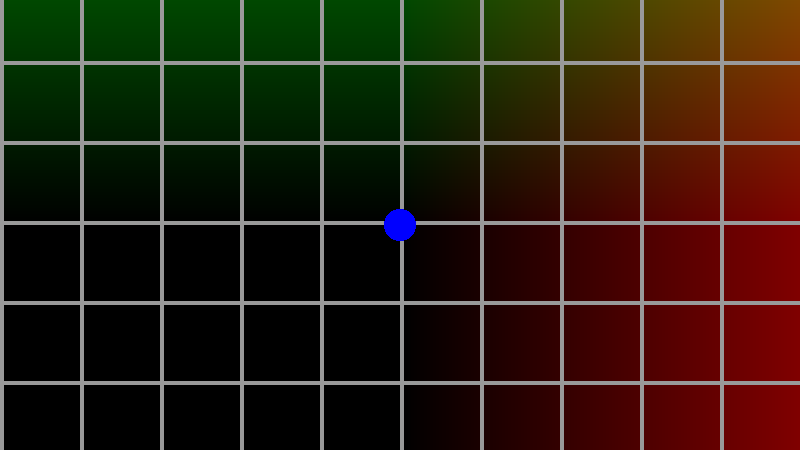
\includegraphics[width=\textwidth]{Plantilla-TFG-master/img/normXColor.png}
        \caption{Eje X}
    \end{minipage}
    \hfill
    \begin{minipage}[b]{0.45\textwidth}
        \centering
        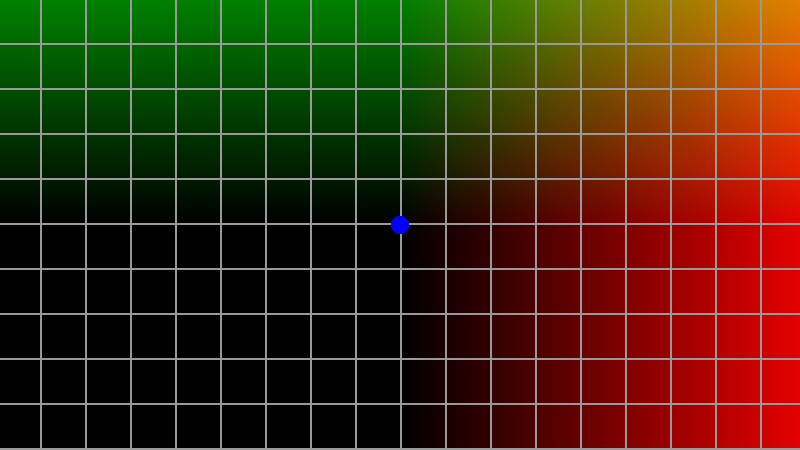
\includegraphics[width=\textwidth]{Plantilla-TFG-master/img/normYColor.png}
        \caption{Eje Y}
    \end{minipage}
    
    \medskip
    
    \begin{minipage}[b]{0.45\textwidth}
        \centering
        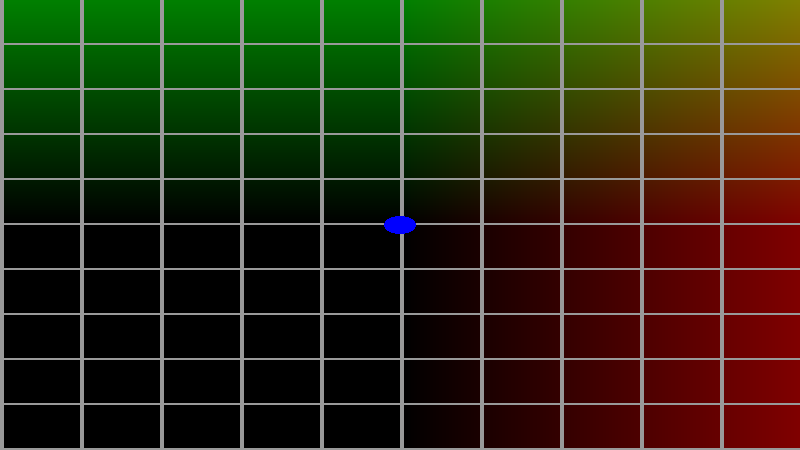
\includegraphics[width=\textwidth]{Plantilla-TFG-master/img/normXYColor.png}
        \caption{Ejes X e Y}
    \end{minipage}
    \hfill
    \begin{minipage}[b]{0.45\textwidth}
        \centering
        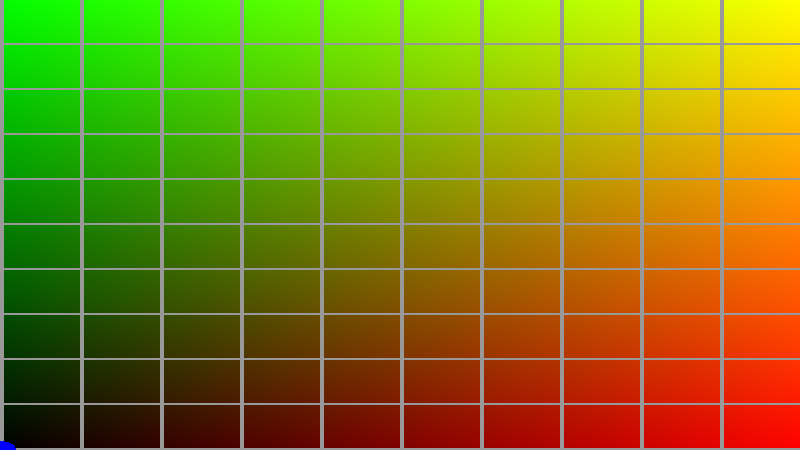
\includegraphics[width=\textwidth]{Plantilla-TFG-master/img/noNormColor.png}
        \caption{Ninguno}
    \end{minipage}
    \caption{Normalización de coordenadas sobre distintos ejes}
    \label{fig:uv}
\end{figure}

Ya tenemos nuestro \textit{fragment shader} preparado para aplicar el algoritmo de \textit{raymarching}: 
\begin{lstlisting}[title=Procesador de fragmentos]
#version 330

void main()
{
    vec2 uv=(gl_FragCoord.xy-.5*u_resolution.xy)/u_resolution.y;
    vec3 color = raymarching(uv);
    gl_FragColor = vec4(color,1.0);
}
\end{lstlisting}

\subsection{Raymarching y Spheretracing}
A partir de ahora, pensamos en que nuestra escena no es la de OpenGL, sino aquella que queremos dibujar usando \textit{raymarching} dado un SDF $\phi$. Podemos pensar en esta escena como $\R^3$ con su base usual $B_u = \{e_1,e_2,e_3\} = \{(1,0,0),(0,1,0),(0,0,1)\}$, donde colocamos los siguientes elementos.
\begin{itemize}
    \item \textbf{Plano de visión:} rejilla en el plano XY y centrada en el origen, donde cada uno de sus cuadrados corresponde a un píxel del lienzo,
    \item \textbf{Punto de la cámara $\boldsymbol{c_o}$:} punto del espacio desde donde se observa la escena,
    \item \textbf{Punto de atención o \textit{lookat point} $\boldsymbol{l}$:} hacia que punto del espacio debe mirar la cámara. Tomaremos siempre $l=(0,0,0)$.
\end{itemize}

El método del \textit{raymarching} consiste en trazar rayos a partir de $c_o$ hacia el centro de cada uno de los cuadrados del plano de visión, de forma que si el rayo interseca con $S_\phi$ significa que ese píxel corresponde a un punto de la superficie, y será coloreado como tal.
\begin{figure}[h]
    \centering
    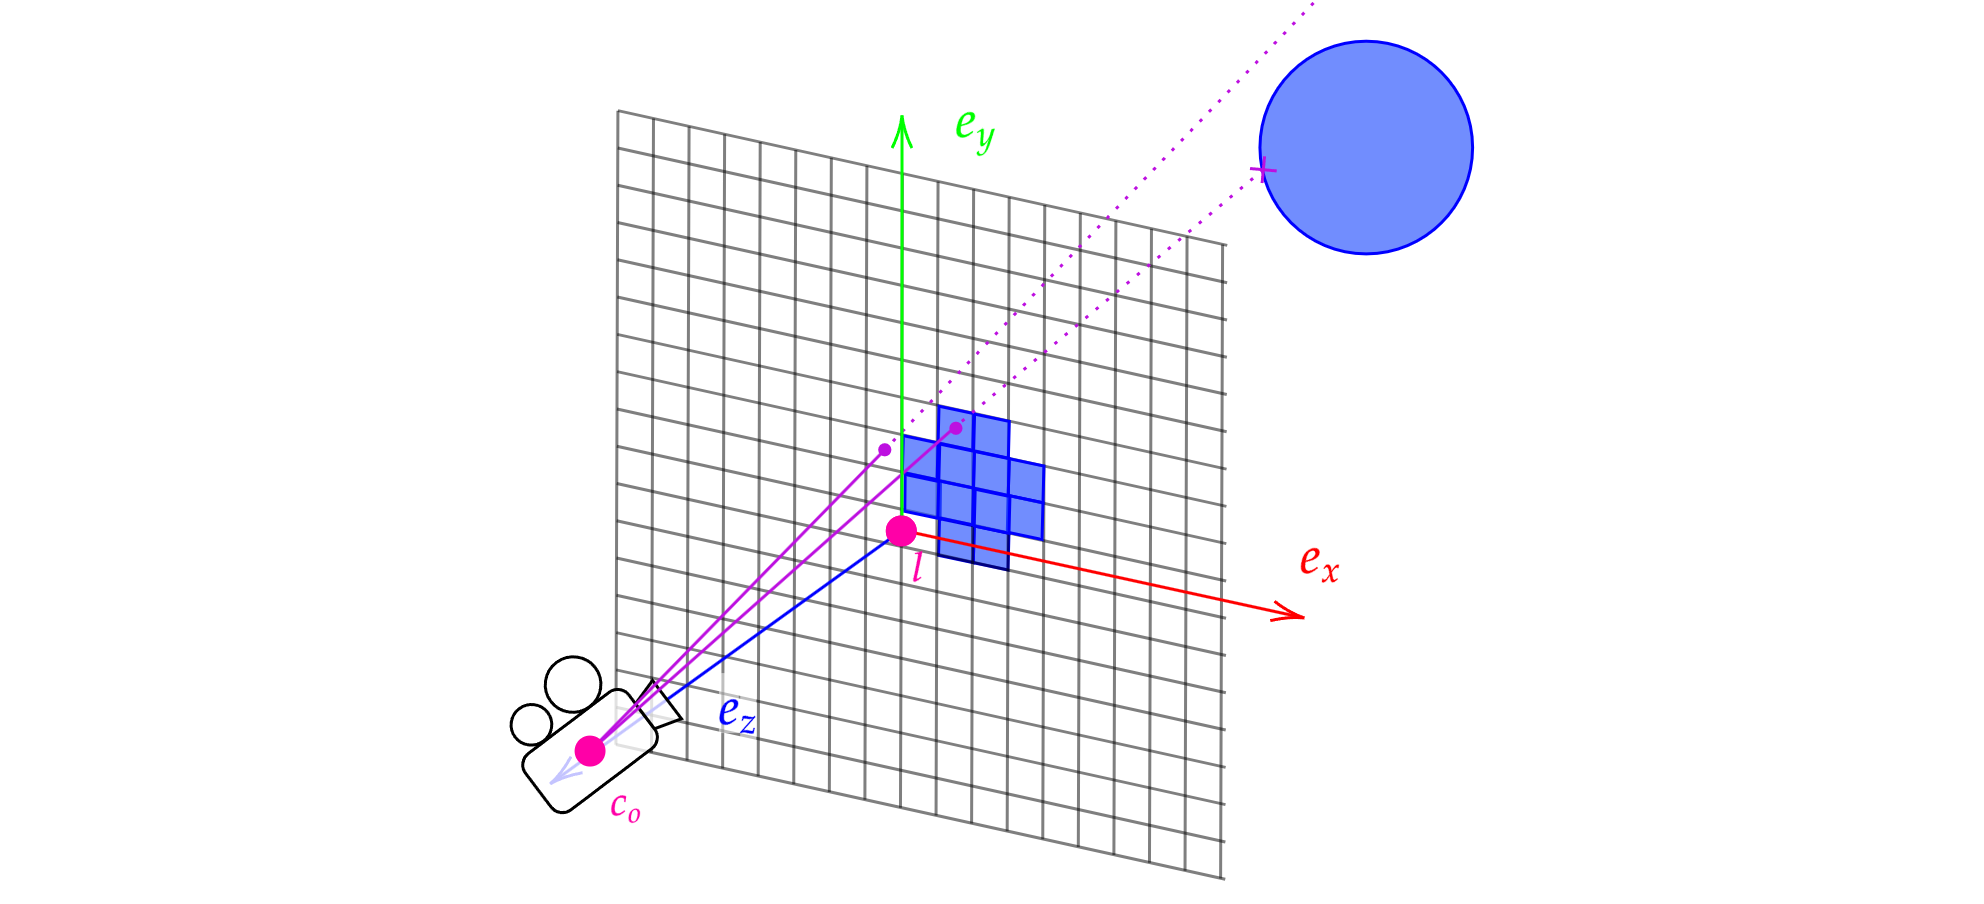
\includegraphics[width=\textwidth]{Plantilla-TFG-master/img/raymarch.png}
    \caption{Trazado de rayos a través del plano de visión}
    \label{fig:raymarch1}
\end{figure}
\newline

Cada uno de estos rayos estará definido por un origen $r_o$ y una dirección $r_d$. El origen será siempre la posición de la cámara $c_o$, pero la dirección requiere más trabajo. En el escenario descrito en la \autoref{fig:raymarch1}, dado que en todo momento conocemos las coordenadas de cada punto de la rejilla a través de $uv = (u,v)$, es claro que podemos tomar $r_d = (u,v,-c_o)$. Aquí $c_o$ actúa como un control del campo de visión, de forma que cuanto menor sea su valor, menor se verán los objetos dibujados. Lo fijaremos a un valor de $1$. Sin embargo este escenario es el más sencillo posible, y si queremos poder mover la cámara tendremos que poder trabajar con una orientación arbitraria suya. Para ello deberemos construir un marco cartesiano relativo a ella, esto es, una base $B=\{f_1,f_2,f_3\}$ de $\R^3$ alineada con la cámara. Esta base deberá ser ortonormal y tener la misma orientación que la base usual. 

Obtenemos primero vectores que nos resultarán útiles para generar esta base.

\begin{itemize}
    \item \textbf{Vector director $\boldsymbol{c_d}$:} indica la dirección hacia la que mirará la cámara. luego vendrá dado por $c_d = l-c_o$,
    \item \textbf{\textit{Right vector} $\boldsymbol{c_r}$ }: es el análogo a $e_x$ en la base usual, luego lo podemos obtener como $c_r = (0,1,0)\times c_d$,
    \item \textbf{\textit{Up vector} $\boldsymbol{c_u}$}: dirección en la que el observador ve proyectada en vertical la escena. Podemos obtenerlo como $c_u = c_d\times c_r$.
\end{itemize}

A partir de estos vectores podemos obtener $\{f_1,f_2,f_3\}$ normalizándolos y teniendo en cuenta que el plano de visión y la cámara estarán orientados de forma opuesta:
\begin{equation*}
    f_1 = -\frac{c_r}{\Vert c_r\Vert} = -\frac{(0,1,0)\times c_d}{\Vert l-c_o\Vert},\quad 
    f_2 = -\frac{c_d}{\Vert c_d\Vert} = -\frac{l-c_o}{\Vert l-c_o\Vert},\quad 
    f_3 = \frac{c_u}{\Vert c_u\Vert } = f_2\times f_1.   
\end{equation*}

Ahora solo queda transformar el vector director $(u,v,-1)$ a la base que acabamos de obtener. La matriz de cambio de base serán las coordenadas por columnas de $\{f_1,f_2,f_3\}$ escritas en función de $\{e_1,e_2,e_3\}$. Al ser esta la base usual, obtenemos que la matriz de cambio de base consiste en escribir por columnas $\{f_1,f_2,f_3\}$, de forma que
\begin{equation*}
    rayo = (u,v,-1)_{B} = (-c_r \vert c_u \vert -c_d) \cdot \begin{pmatrix}
        u\\
        v\\
        -1
    \end{pmatrix}
\end{equation*}

\begin{figure}[ht!]
    \centering
    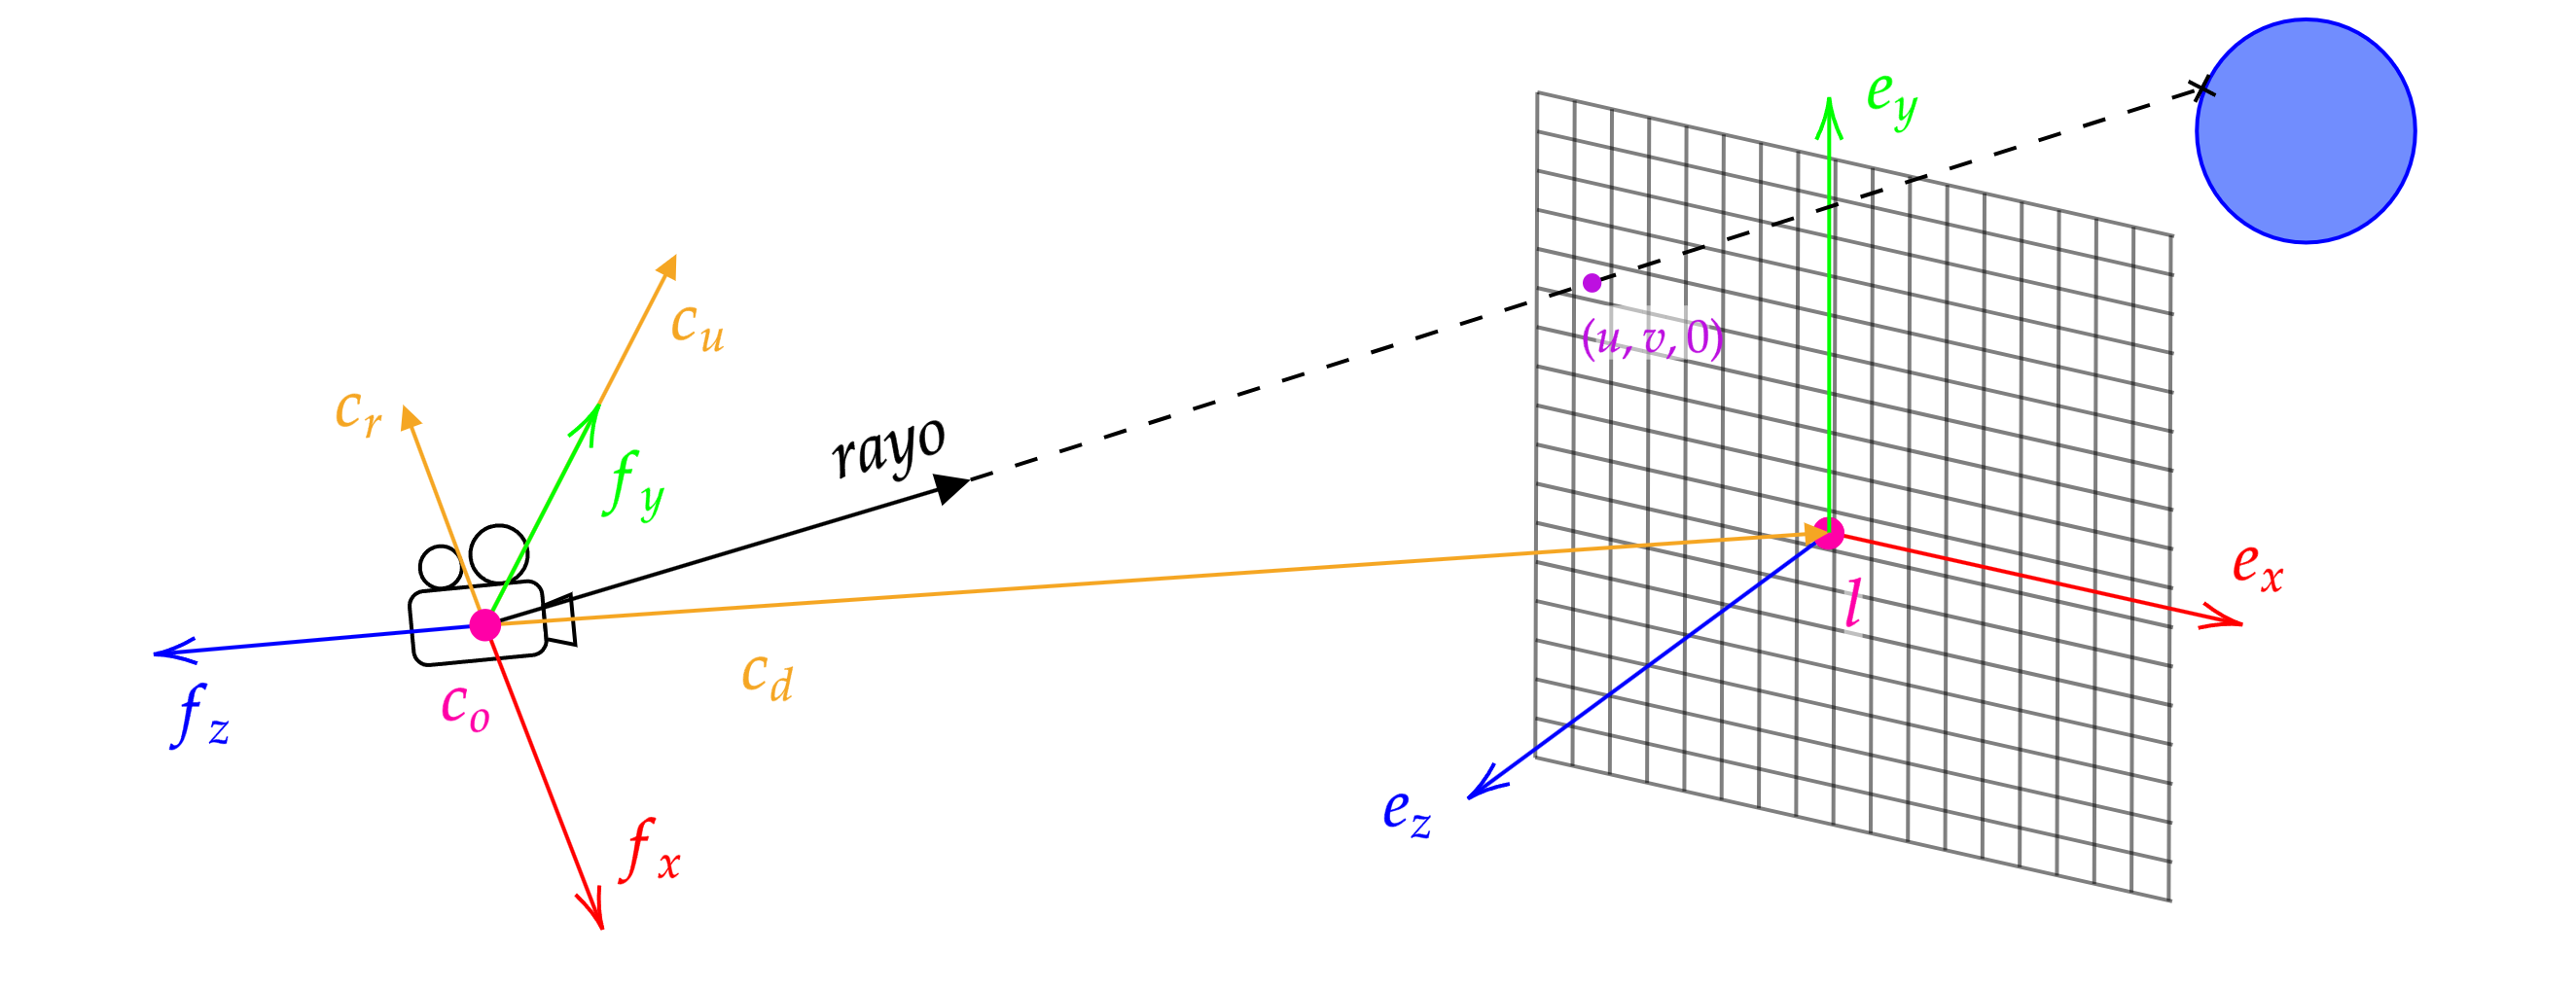
\includegraphics[width=\textwidth]{Plantilla-TFG-master/img/raydir.png}
    \caption{Obtención de la dirección del rayo}
    \label{fig:raydir}
\end{figure}

Ahora que ya tenemos toda la información del rayo, falta comprobar si este interseca con $S_{\phi}$. Para esto se utiliza un método iterativo: a partir de $c_o$, en cada iteración avanzamos en la dirección del rayo una distancia fija $\delta$. Evaluamos entonces nuestro SDF en la posición actual, de forma que si obtenemos un valor muy cercano a $0$ significará que hemos llegado a la isosuperficie. De lo contrario, repetimos el proceso hasta encontrar una intersección o superar un número máximo de iteraciones, en cuyo caso concluiremos que no hay intersección. La \autoref{a:raymarching} ilustra este procedimiento, donde \texttt{DibujarSuperficie()} y \texttt{DibujarFondo()} devuelven ternas RGBA que serán asignadas al píxel actual dependiendo de si hay intersección o no.\newline

\begin{figure}[ht!]
    \centering
    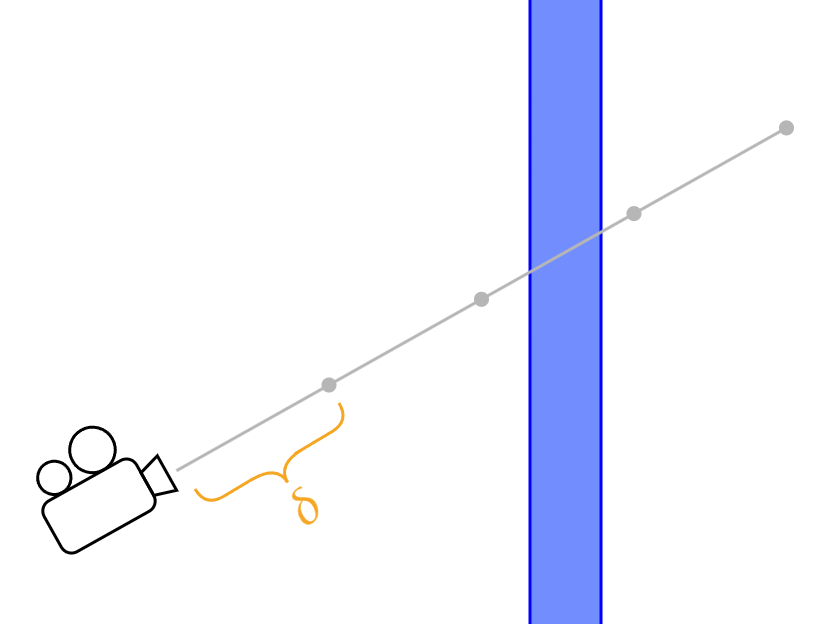
\includegraphics[width=0.5\textwidth]{Plantilla-TFG-master/img/miss.png}
    \caption{Pérdida de intersección en \textit{raymarching} para valores elevados de $\delta$}
    \label{fig:miss}
\end{figure}

\SetKwComment{Comment}{// }{}
\begin{figure}[ht!]
    \centering
    \begin{minipage}{0.50\textwidth}
        \begin{algorithm}[H]
            \caption{Raymarching}
                \KwData{origen $p$, dirección $v$}
                
                $d \gets 0$ \Comment{distancia total}
                
                \For{i $\in$ MAX\_ITERACIONES} {
                    rayo $\gets p +d\cdot v$
                    
                    sdf $\gets \phi(\text{rayo})$
                    
                    \If{sdf $< \varepsilon$}{
                       \Return{DibujarSuperficie(rayo)}
                    }
            
                    $d\gets d + \delta$\;
            
                    \If{$d >$ MAX\_DISTANCIA}{
                        \Return{DibujarFondo()}
                    }
                }
        \end{algorithm}
    \end{minipage}%
    \hfill
    \begin{minipage}{0.48\textwidth}
        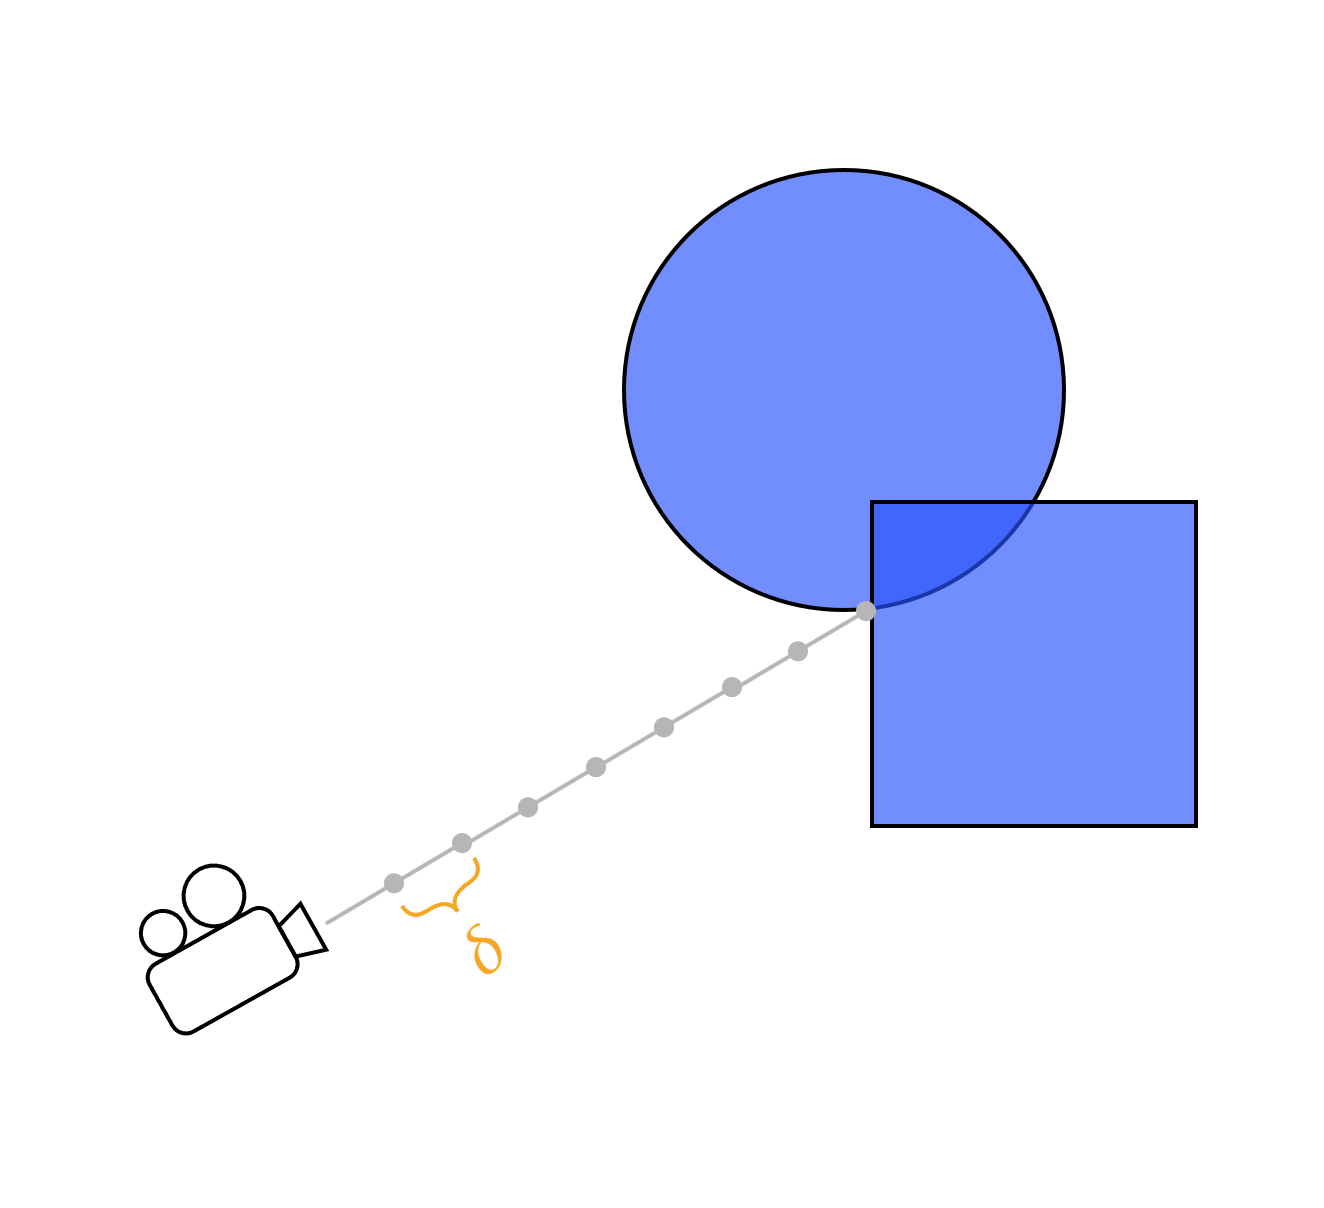
\includegraphics[width=\textwidth]{raymarching.png}
    \end{minipage}
    \caption{Algoritmo de \textit{raymarching}}
    \label{a:raymarching}
\end{figure}

Una desventaja de esta técnica es que puede ser bastante lenta, ya que cuanto más alejados estén los puntos de $S_\phi$ del observador, mayor es el número de iteraciones necesarias para encontrar la intersección en caso de que la haya. En el peor de los casos en el que tal intersección no exista, se habrá realizado el número máximo de iteraciones, que deberá ser bastante alto, pues si no queremos perder ninguna intersección como ocurre en la \autoref{fig:miss}, el valor de incremento $\delta$ tenddrá que ser pequeño.\newline

La solución a este problema es el uso de \textit{spheretracing}, que reduce drásticamente el número de iteraciones y por tanto evaluaciones de $\phi$, necesarias para detectar la intersección. Su funcionamiento es similar al \textit{raymarching}, con la diferencia de que el incremento en la posición del rayo no es fija, sino que es la máxima que podemos tomar en cada momento asegurándonos de no perder información. Esta distancia será la mínima del punto actual del rayo a $S_\phi$, que no es más que evaluar $\phi$ en dicho punto.\newline

El algoritmo que usaremos será por tanto el descrito en la \autoref{a:spheretracing}. 
\begin{figure}[ht!]
    \centering
    \begin{minipage}{0.50\textwidth}
       \begin{algorithm}[H]
            \caption{Spheretracing}
                \KwData{origen $p$, dirección $v$}
                $d \gets 0$ \Comment{distancia actual}
                
                \For{i $\in$ MAX\_ITERACIONES} {
                    rayo $\gets p + d \cdot v$
                    
                    sdf $\gets \phi(\text{rayo})$
                    
                    \If{sdf $< \varepsilon$}{
                       \Return{DibujarSuperficie(rayo)};
                    }
            
                    $d \gets$ d + sdf
            
                    \If{$d >$ MAX\_DISTANCIA}{
                        \Return{DibujarFondo()};
                    }
                }
        \end{algorithm}
    \end{minipage}%
    \hfill
    \begin{minipage}{0.48\textwidth}
        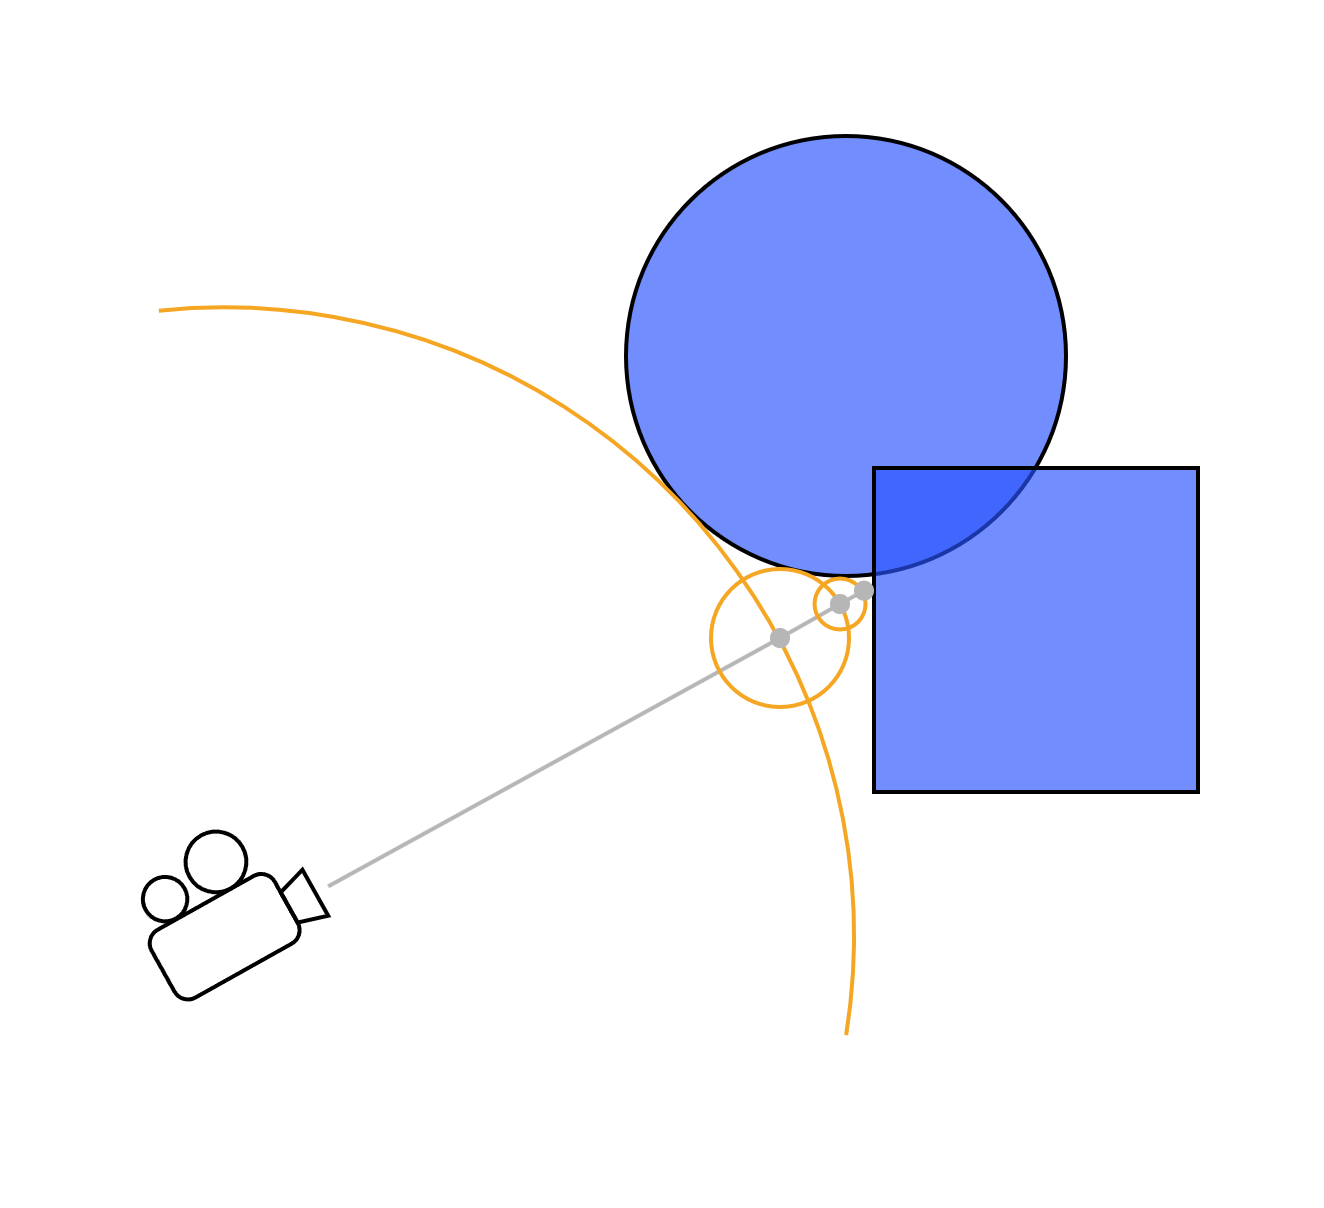
\includegraphics[width=\textwidth]{spheremarching.png}
    \end{minipage}
    \caption{Algoritmo de \textit{spheretracing}}
    \label{a:spheretracing}
\end{figure}

\subsection{Iluminación}
Ya sabemos qué píxeles pertenecen a la superficie, pero no de qué color deben dibujarse. Para ello utilizaremos el modelo de reflexión de Phong. En él trabajaremos con los siguientes parámetros:
\begin{itemize}
  \item Luz ambiente $i_a$: vector RGB suma de las contribuciones de todas las fuentes de luz de la escena. Contiene un valor por defecto que será el color del fondo.
  \item Lista de fuentes de luz $(l_1, \dots, l_m, \dots, l_n)$.
  \item Materiales asignados a cada objeto definidos por las constantes:
      \begin{itemize}
          \item Reflexión especular $k_s$: modela cómo se refleja la luz en objetos brillantes. Depende tanto de la posición de las fuentes de luz como de la del observador.
          \item Reflexión difusa $k_d$: modela cómo se refleja la luz en objetos mates. Depende de la posición de las fuentes de luz, pero no de la posición del observador.
          \item Reflexión ambiental $k_a$: representa la proporción de luz del ambiente que refleja el objeto.
          \item Coeficiente de brillo $\alpha$: valor real positivo que permite variar el tamaño de las zonas brillantes (a mayor valor, menor tamaño y más pulida o especular).
      \end{itemize}
  
  \item Los vectores normalizados definidos para cada punto de la superficie $p$:
        \begin{itemize}
          \item $L_m$: vector director desde $p$ a cada fuente de luz $l_m$.
          \item $N$ vector normal a la superficie en $p$.
          \item $R_m$ dirección del rayo de luz reflejado especularmente desde la fuente $l_m$ en el punto $p$.
          \item $V$: dirección de $p$ a la posición del observador.
        \end{itemize}
\end{itemize}

TODO: diagrama vectores

Con estas variables, el color en $p$ vendrá dado por la fórmula:
\begin{equation*}
  I_p = k_a i_a + \sum_{m=0}^{n} \left(k_d\left(L_m\cdot N\right) + k_s\left(R_m\cdot V\right)^{\alpha} \right)
\end{equation*}

De los vectores anteriores, $L_m$ y $V$ se calculan trivialmente, y $R_m$ se puede obtener como
\begin{equation*}
  R_m = 2(L_m\cdot N)N - L_m
\end{equation*}

Veamos como obtener $N$.

\subsubsection{Cálculo del vector normal}
\begin{definicion}
  El \textbf{gradiente} de una función implícita $\phi\colon \R^3\to\R$ es $\nabla\phi = \left(\frac{\partial \phi}{\partial x}, \frac{\partial \phi}{\partial y}, \frac{\partial \phi}{\partial z}\right)$.
\end{definicion}

\begin{proposicion}\label{p:gradient_perp}
  $\nabla\phi$ es perpendicular a $S_\phi$.
\end{proposicion}

\begin{proof}
  Sea $s\in S_\phi$ arbitrario. Tomamos una curva parametrizada:
  \begin{align*}
    \alpha \colon [0,1] & \to S_\phi                             \\
    t                   & \mapsto \left(x(t), y(t), z(t) \right)
  \end{align*}

  cumpliendo $\alpha(t_0)=s$. Veamos que $\nabla\phi(s) \perp \alpha$:

  \begin{align*}
    \alpha(t)\subset S_\phi & \implies \phi(\alpha(t))=0\\
                            & \implies \nabla\phi(\alpha(t)) = \frac{\partial{F}}{\partial{x}}\frac{dx}{dt} + \frac{\partial{F}}{\partial{y}}\frac{dy}{dt} + \frac{\partial{F}}{\partial{z}}\frac{dz}{dt} = 0 \\
                            & \implies \langle \nabla\phi(x,y,z), \alpha'(t)\rangle = 0 \implies \langle \nabla\phi(x,y,z), \alpha'(t_0)\rangle = 0
  \end{align*}

    Por tanto, $\nabla\phi(s)$ es perpendicular al vector tangente de $\alpha$ en $s$, que a su vez está contenida en el plano tangente de $S_\phi$ en $s$. Por tanto $\nabla\phi(s) \perp S_\phi$.
\end{proof}

Hemos visto que calcular $N$ equivale a calcular $\nabla\phi$. Sin embargo, dado que la superficie viene dada por un SDF que podría ser no derivable, no podemos hacerlo de forma analítica. De ser derivable, podría ser una buena opción calcular el gradiente una única vez al momento de definir la $\phi$, tras lo cual para obtener $N$ solo habría que realizar evaluaciones de dicho gradiente. Sin embargo, por su sencillez y popularidad, nos decantaremos por un método numérico que únicamente hará uso de evaluaciones de $\phi$.

\begin{definicion}
  Dada $\phi:\R^3\to \R$ diferenciable, $p = (x,y,z)$, $v\in \R^3$, definimos la \textbf{derivada direccional} en $p$ con dirección $v$ a:
  \begin{equation*}
    \nabla_v f(p) = \nabla f(p) \cdot v = \frac{\partial{f}(p)}{\partial{x}}v_x + \frac{\partial{f}(p)}{\partial{y}}v_y + \frac{\partial{f}(p)}{\partial{z}}v_z
  \end{equation*}
\end{definicion}

Para el cálculo de cada parcial de $f$ podemos utilizar la definición de derivada. Por ejemplo, para la primera componente:
\begin{equation*}
  \frac{\partial{f}(p)}{\partial{x}} v_x = \lim_{h\to 0}\frac{f(p + (h,0,0)) - f(p)}{h} v_x
\end{equation*}

Procedemos a calcular $N$ aplicaremos el \textbf{método del tetraedro}, el cual se basa en evaluar $\phi$ en la dirección de los vértices de un tetraedro:

\begin{equation*}
    k_0 = (1,-1,-1)\quad k_1 = (-1,-1,1)\quad k_2=(-1,1,-1)\quad k_3=(1,1,1)
\end{equation*}

\begin{proposicion}[Método del tetraedro]
  Dado $p\in S_\phi$, su vector normal $N$ se obtiene normalizando el vector
  \begin{equation*}
    \hat{N} = \sum_{i=0}^3 k_i\cdot f(p + hk_i)
  \end{equation*}
\end{proposicion}

\begin{proof}
  Por la proposición \autoref{p:gradient_perp}, basta comprobar que $\hat{N}$ es colineal a $\nabla \phi(p)$.

  \begin{align*}
    \hat{N} & = \sum_{i=0}^3 k_i\cdot f(p + hk_i) = \sum_{i=0}^3 k_i\cdot f(p + hk_i) + k_i\cdot f(p) = \sum_{i=0}^3 k_i\cdot f(p+hk_i - f(p)) = \sum_{i=0}^3 k_i \nabla_{k_i}f(x)\\
    &= \sum_{i=0}^3 k_i \cdot \left( k_i \cdot \nabla f(p)\right) = \sum_{i=0}^3 (k_i\cdot k_i) \nabla f(p) = \sum_{i=0}^3 \nabla f(p) = 4\nabla f(p)
  \end{align*}

  donde hemos usado que $\sum_{i=0}^3 k_i = (0,0,0)$, $\sum_{i=0}^3 k_i\cdot k_i = (1,1,1)$, y que el producto escalar es un operador lineal.
\end{proof}

\section{Aproximación de implícitas}
Empezábamos el capítulo diciendo que una de las representaciones más comunes de superficies es a través de implícitas, pero hasta ahora nos hemos centrado en estudiar un tipo particular de este tipo de ecuaciones. Si intentásemos aplicar los algoritmos anteriores a una función implícita cualquiera, observaríamos que el resultado tiene ciertos defectos, tales como deformaciones, o incluso no se visualiza. Vamos a introducir una técnica que dada una función implícita $\phi$, nos permitirá obtener un SDF aproximado de $S_\phi$. Esto nos será útil cuando no conozcamos o no podamos calcular explícitamente el SDF de una superficie pero sí su representación implícita.

\begin{proposicion}
    Sea $\phi\colon \R^3\to\R$ una función implícita cualquiera y $p\in\R^3$. Entonces: 
    \begin{equation*}    
        \sdf_{S_\phi}(p) \approx \frac{\vert \phi(p)\vert}{\vert \nabla\phi(p)\vert}
    \end{equation*}
\end{proposicion}
\begin{proof}
    Sea $q$ al punto de $S_\phi$ más cercano a $p$ y $v=\vec{pq} \perp S_\phi$ en $q$. Queremos calcular la distancia de $p$ a $S_\phi$, que es justamente $v$. Podemos calcular el desarrollo de Taylor de $\phi$ en $p$:
    \begin{equation*}
        \phi(p+v) = \phi(p) + \nabla(p)\cdot (p+v-p) + \mathcal{O}(\vert p+v-p\vert^2) \implies \phi(p+v) = \phi(p) + \nabla(p)\cdot v + \mathcal{O}(\vert v\vert^2)
    \end{equation*}

    Suponemos ahora que $p$ está cerca de $S_\phi$, esto es, $\vert v\vert < \varepsilon$. Como $\phi(p+v) = \phi(q)=0$, tenemos que:
    \begin{align*}
        0 &= \vert \phi(p+v)\vert \approx \vert \phi(p) + \nabla(p)\cdot v \vert \le \vert \phi(p)\vert - \vert \nabla(p)\cdot v \vert\\
         &\le \vert \phi(p)\vert - \vert \nabla(p)\vert \vert v \vert \implies \vert v\vert \le \frac{\vert \phi(p)\vert}{\vert \nabla(p)\vert}
    \end{align*}
    donde hemos usado la desigualdad triangular y las propiedades del producto escalar.
\end{proof}

Al igual que nos ocurría al calcular el vector normal, habrá ocasiones en las que el gradiente no pueda ser obtenido de forma analítica. Esta vez sin embargo no nos basta con conocer solo la dirección del gradiente, así que no podemos aplicar de nuevo el método del tetraedro. Usaremos un nuevo método en su lugar que usa la definición de derivada.

\begin{proposicion}[Método de las diferencias centrales]
    Sea $\phi\colon \R^3\to\R$. Entonces:
    \begin{align*}
        \frac{\partial\phi}{\partial x}(p) &\approx \frac{\phi(p+(h,0,0)) - \phi(p-(h,0,0))}{2h}\\[10pt]
        \frac{\partial\phi}{\partial y}(p) &\approx \frac{\phi(p+(0,h,0)) - \phi(p-(0,h,0))}{2h}\\[10pt]
        \frac{\partial\phi}{\partial z}(p) &\approx \frac{\phi(p+(0,0,h)) - \phi(p-(0,0,h))}{2h}
    \end{align*}
    
    donde $h\in\R^+$ es un valor arbitrariamente pequeño. 
\end{proposicion}

Para calcular el gradiente necesitaremos evaluar $\phi$ un total de seis veces, ya que hay que realizar dos evaluaciones por cada variable. Es por este motivo que 





% !TeX root = ../libro.tex
% !TeX encoding = utf8

\chapter{Desarrollo e implementación}
Nos centramos ahora en los aspectos de la implementación de una aplicación que haga uso de todas las técnicas y conceptos tratados en los capítulos anteriores. Para ello, se ha usado \href{https://es.reactjs.org/}{React}, una biblioteca de JavaScript (y TypeScript) para interfaces de usuario. Las principales ventajas de este enfoque son:
\begin{itemize}
    \item La aplicación puede ser ejecutada en cualquier navegador, haciendo que sea mucho más accesible.
    \item React está basada en componentes modulares, lo que la hace escalable. Además. debido a su popularidad, hay una infinidad de librerías de terceros a nuestra disposición, ya sea específicas de React o de JavaScript.
\end{itemize}

Un aspecto fundamental a lo largo de todo el desarrollo será el del rendimiento. Esto es debido a que, por defecto, las aplicaciones web solo tienen a su disposición una hebra de ejecución (la de interfaz de usuario), haciendo de cuello de botella para el resto de cálculos.

\section{Librería de polinomios multivariable}
Si bien tenemos a nuestra disposición un gran número de librerías externas, en el momento de realización de la aplicación no encontré ninguna alternativa viable para trabajar con polinomios multivariable en JavaScript de forma nativa. Como alternativas se barajó el uso de la API de \href{https://wiki.geogebra.org/en/Reference:GeoGebra_Apps_API}{Geogebra} o realizar llamadas a código Python que usara \href{https://www.sagemath.org/}{SageMath}. Sin embargo, por motivos de rendimiento y completitud, se decidió desarrollar una librería nativa en TypeScript para el manejo de polinomios en varias variables y cálculo de bases de Groebner. Se encuentra disponible en \href{https://github.com/Daniel2000815/multivariate-polynomial}{GitHub} junto a su documentación, ejemplos de uso y tests usados.\newline

La librería consta de tres clases que pasamos a estudiar a continuación.

\subsection{Clase \texttt{Monomial}}

\subsection{Clase \texttt{Polynomial}}

\subsection{Clase \texttt{Ideal}}
% !TeX root = ../libro.tex
% !TeX encoding = utf8

\chapter{Desarrollo e implementación}
Nos centramos ahora en los aspectos de la implementación de una aplicación que haga uso de todas las técnicas y conceptos tratados en los capítulos anteriores. Para ello, se ha usado \href{https://es.reactjs.org/}{React}, una biblioteca de JavaScript (y TypeScript) para interfaces de usuario. Las principales ventajas de este enfoque son:
\begin{itemize}
    \item La aplicación puede ser ejecutada en cualquier navegador, haciendo que sea mucho más accesible.
    \item React está basada en componentes modulares, lo que la hace escalable. Además. debido a su popularidad, hay una infinidad de librerías de terceros a nuestra disposición, ya sea específicas de React o de JavaScript.
\end{itemize}

Un aspecto fundamental a lo largo de todo el desarrollo será el del rendimiento. Esto es debido a que, por defecto, las aplicaciones web solo tienen a su disposición una hebra de ejecución (la de interfaz de usuario), haciendo de cuello de botella para el resto de cálculos.

\section{Librería de polinomios multivariable}
Si bien tenemos a nuestra disposición un gran número de librerías externas, en el momento de realización de la aplicación no encontré ninguna alternativa viable para trabajar con polinomios multivariable en JavaScript de forma nativa. Como alternativas se barajó el uso de la API de \href{https://wiki.geogebra.org/en/Reference:GeoGebra_Apps_API}{Geogebra} o realizar llamadas a código Python que usara \href{https://www.sagemath.org/}{SageMath}. Sin embargo, por motivos de rendimiento y completitud, se decidió desarrollar una librería nativa en TypeScript para el manejo de polinomios en varias variables y cálculo de bases de Groebner. Se encuentra disponible en \href{https://github.com/Daniel2000815/multivariate-polynomial}{GitHub} junto a su documentación, ejemplos de uso y tests usados.\newline

La librería consta de tres clases que pasamos a estudiar a continuación.

\subsection{Clase \texttt{Monomial}}

\subsection{Clase \texttt{Polynomial}}

\subsection{Clase \texttt{Ideal}}

% --------------------------------------------------------------------
% APPENDIX: Opcional
% --------------------------------------------------------------------

\appendix % Reinicia la numeración de los capítulos y usa letras para numerarlos
%\pdfbookmark[-1]{Apéndices}{appendix} % Alternativamente podemos agrupar los apéndices con un nuevo \part{Apéndices}

% !TeX root = ../libro.tex
% !TeX encoding = utf8

\chapter{Resultados de operaciones sobre SDF}\label{ap:operacionesSDF}

TODO

\endinput
%------------------------------------------------------------------------------------
% FIN DEL APÉNDICE. 
%------------------------------------------------------------------------------------

% Añadir tantos apéndices como sea necesario 

% --------------------------------------------------------------------
% GLOSARIO: Opcional
% --------------------------------------------------------------------

%% !TeX root = ../libro.tex
% !TeX encoding = utf8

\chapter*{Glosario}
\addcontentsline{toc}{chapter}{Glosario} % Añade el glosario a la tabla de contenidos

La inclusión de un glosario es opcional.

Archivo: \texttt{glosario.tex}

\begin{description} 
  \item[$\mathbb{R}$] Conjunto de números reales.

  \item[$\mathbb{C}$] Conjunto de números complejos.

  \item[$\mathbb{Z}$] Conjunto de números enteros.
\end{description}
\endinput


% -------------------------------------------------------------------
% BACKMATTER
% -------------------------------------------------------------------

\backmatter % Desactiva la numeración de los capítulos
\pdfbookmark[-1]{Referencias e Índices}{BM-Referencias}

% BIBLIOGRAFÍA
%-------------------------------------------------------------------
\bibliographystyle{ieeetr}
\begin{small} % Normalmente la bibliografía se imprime en un tamaño de letra más pequeño.

  \bibliography{library.bib}
\end{small}


% ÍNDICE TERMINOLÓGICO  (Opcional) 
%------------------------------------------------------------------- 

% Para incluir el índice terminológico es necesario descomentar los siguientes comandos. Incluir un índice terminológico es opcional

% \cleardoublepage 
% \begin{footnotesize} % Normalmente el índice se imprime en un tamaño de letra más pequeño.
% \printindex 
% \end{footnotesize}

\end{document}
